\documentclass{article}

\usepackage{fancyhdr} % Required for custom headers
\usepackage{lastpage} % Required to determine the last page for the footer
\usepackage{extramarks} % Required for headers and footers
\usepackage[usenames,dvipsnames]{color} % Required for custom colors
\usepackage{graphicx} % Required to insert images
\usepackage{listings} % Required for insertion of code
\usepackage{courier} % Required for the courier font
\usepackage{lipsum} % Used for inserting dummy 'Lorem ipsum' text into the template
\usepackage{amsmath}
\usepackage{amssymb}
\usepackage{mathtools, xparse}
\usepackage{booktabs}
\usepackage{bigstrut}
\usepackage{float}
\usepackage{hyperref}
\usepackage{color}
\usepackage{algorithm}
%\usepackage{caption}
\usepackage{algpseudocode}
\usepackage{multirow}
\usepackage{subfigure}
\usepackage{longtable}
\usepackage{supertabular}

\DeclarePairedDelimiter{\norm}{\lVert}{\rVert}
\DeclarePairedDelimiter\abs{\lvert}{\rvert}%

\hypersetup{
    colorlinks   = true,    % Colours links instead of ugly boxes
    urlcolor     = red,    % Colour for external hyperlinks
    linkcolor    = red,    % Colour of internal links
    citecolor    = red      % Colour of citations
}
% Margins
\topmargin=-0.45in
\evensidemargin=0in
\oddsidemargin=0in
\textwidth=6.5in
\textheight=9.0in
\headsep=0.25in

\linespread{1.1} % Line spacing

% Set up the header and footer
\pagestyle{fancy}
\lhead{\hmwkAuthorName} % Top left header
\chead{\hmwkClass\ : \hmwkID} % Top center head
\rhead{\firstxmark} % Top right header
\lfoot{\lastxmark} % Bottom left footer
\cfoot{} % Bottom center footer
\rfoot{Page\ \thepage\ of\ \protect\pageref*{LastPage}} % Bottom right footer
\renewcommand\headrulewidth{0.4pt} % Size of the header rule
\renewcommand\footrulewidth{0.4pt} % Size of the footer rule

\setlength\parindent{0pt} % Removes all indentation from paragraphs

%----------------------------------------------------------------------------------------
%	CODE INCLUSION CONFIGURATION
%----------------------------------------------------------------------------------------

\definecolor{MyDarkGreen}{rgb}{0.0,0.4,0.0} % This is the color used for comments
\lstloadlanguages{Perl} % Load Perl syntax for listings, for a list of other languages supported see: ftp://ftp.tex.ac.uk/tex-archive/macros/latex/contrib/listings/listings.pdf
\lstset{language=Perl, % Use Perl in this example
    frame=single, % Single frame around code
    basicstyle=\small\ttfamily, % Use small true type font
    keywordstyle=[1]\color{Blue}\bf, % Perl functions bold and blue
    keywordstyle=[2]\color{Purple}, % Perl function arguments purple
    keywordstyle=[3]\color{Blue}\underbar, % Custom functions underlined and blue
    identifierstyle=, % Nothing special about identifiers                                         
    commentstyle=\usefont{T1}{pcr}{m}{sl}\color{MyDarkGreen}\small, % Comments small dark green courier font
    stringstyle=\color{Purple}, % Strings are purple
    showstringspaces=false, % Don't put marks in string spaces
    tabsize=5, % 5 spaces per tab
    %
    % Put standard Perl functions not included in the default language here
    morekeywords={rand},
    %
    % Put Perl function parameters here
    morekeywords=[2]{on, off, interp},
    %
    % Put user defined functions here
    morekeywords=[3]{test},
    %
    morecomment=[l][\color{Blue}]{...}, % Line continuation (...) like blue comment
    numbers=left, % Line numbers on left
    firstnumber=1, % Line numbers start with line 1
    numberstyle=\tiny\color{Blue}, % Line numbers are blue and small
    stepnumber=5 % Line numbers go in steps of 5
}

% Creates a new command to include a perl script, the first parameter is the filename of the script (without .pl), the second parameter is the caption
\newcommand{\perlscript}[2]{
    \begin{itemize}
        \item[]\lstinputlisting[caption=#2,label=#1]{#1.py}
    \end{itemize}
}
\newcommand{\cppscript}[1]{
    \begin{itemize}
        \item[]\lstinputlisting[]{#1}
    \end{itemize}
}

%----------------------------------------------------------------------------------------
%	DOCUMENT STRUCTURE COMMANDS
%	Skip this unless you know what you're doing
%----------------------------------------------------------------------------------------

% Header and footer for when a page split occurs within a problem environment
\newcommand{\enterProblemHeader}[1]{
    \nobreak\extramarks{#1}{#1 continued on next page\ldots}\nobreak
    \nobreak\extramarks{#1 (continued)}{#1 continued on next page\ldots}\nobreak
}

% Header and footer for when a page split occurs between problem environments
\newcommand{\exitProblemHeader}[1]{
    \nobreak\extramarks{#1 (continued)}{#1 continued on next page\ldots}\nobreak
    \nobreak\extramarks{#1}{}\nobreak
}

%\setcounter{secnumdepth}{0} % Removes default section numbers
\newcounter{homeworkProblemCounter} % Creates a counter to keep track of the number of problems

\newcommand{\homeworkProblemName}{}
\newenvironment{homeworkProblem}[1][Problem \arabic{homeworkProblemCounter}]{ % Makes a new environment called homeworkProblem which takes 1 argument (custom name) but the default is "Problem #"
    \stepcounter{homeworkProblemCounter} % Increase counter for number of problems
    \renewcommand{\homeworkProblemName}{#1} % Assign \homeworkProblemName the name of the problem
    \section{\homeworkProblemName} % Make a section in the document with the custom problem count
    \enterProblemHeader{\homeworkProblemName} % Header and footer within the environment
    }{
    \exitProblemHeader{\homeworkProblemName} % Header and footer after the environment
}

\newcommand{\problemAnswer}[1]{ % Defines the problem answer command with the content as the only argument
\noindent\framebox[\columnwidth][c]{\begin{minipage}{0.98\columnwidth}#1\end{minipage}} % Makes the box around the problem answer and puts the content inside
}

\newcommand{\homeworkSectionName}{}
\newenvironment{homeworkSection}[1]{ % New environment for sections within homework problems, takes 1 argument - the name of the section
    \renewcommand{\homeworkSectionName}{#1} % Assign \homeworkSectionName to the name of the section from the environment argument
    \subsection{\homeworkSectionName} % Make a subsection with the custom name of the subsection
    \enterProblemHeader{\homeworkProblemName\ [\homeworkSectionName]} % Header and footer within the environment
    }{
    \enterProblemHeader{\homeworkProblemName} % Header and footer after the environment
}

%----------------------------------------------------------------------------------------
%	NAME AND CLASS SECTION
%----------------------------------------------------------------------------------------

\newcommand{\hmwkID}{homework 11} % Assignment title
\newcommand{\hmwkTitle}{Diode Networks}
\newcommand{\hmwkDueDate}{Tuesday,\ May\ 16,\ 2017} % Due date
\newcommand{\hmwkClass}{Numerical Analysis} % Course/class
\newcommand{\hmwkClassTime}{10:30am} % Class/lecture time
\newcommand{\hmwkClassInstructor}{Jones} % Teacher/lecturer
\newcommand{\hmwkAuthorName}{102061149 Fu-En Wang} % Your name

%----------------------------------------------------------------------------------------
%	TITLE PAGE
%----------------------------------------------------------------------------------------

\title{
    \vspace{2in}
    \textmd{\textbf{\hmwkClass}}\\
    \textmd{\textbf{\hmwkID: \hmwkTitle}} \\
    \normalsize\vspace{0.1in}\small{Due\ on\ \hmwkDueDate}\\
    \vspace{3in}
}

\author{\textbf{\hmwkAuthorName}}
\date{} % Insert date here if you want it to appear below your name

%----------------------------------------------------------------------------------------

\begin{document}
\maketitle
\newpage

\section{Introduction}
To calculate the current of a diode, the formula is:
\begin{align}
    & i_d = I_s(e^{\frac{v_d}{\phi}} - 1) \\
    & \phi = \frac{\phi_0T}{300}
\end{align}
where $I_s$ is 1 Amps, $\phi_0$ is 0.026 Volts and $v_d$ is the cross-voltage of diode.

In this homework, we will build a Non-linear System to analyze the following diode network.
\begin{figure}[H]
    \centering
    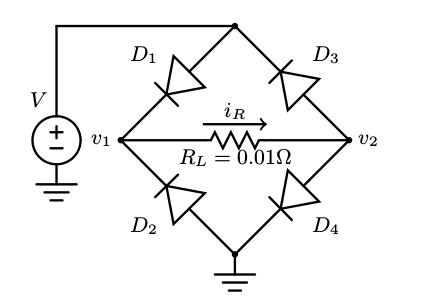
\includegraphics[width=0.45\textwidth]{src/diode-network.jpg}
    \caption{Simple Diode Network}
    \label{fig:diode-network}
\end{figure}
To build a robust function to solve any non-linear system, I use \textbf{Finite Difference Approximation} to calculate Jacobian matrix
\begin{align}
    \frac{\partial{F}}{\partial{x}} = \frac{F(x+h) - F(x)}{h}
\end{align}

\subsection{Problems}
In this homework, we need to solve two problems: \newline

1. With temperature fixed at 300k, find $v1$, $v2$, $i_{D1}$ , $i_{D2}$, $i_{D3}$, $i_{D4}$ and $i_R$ when V = -1.0, -0.98,....., 1 Volt. \newline
\newline
2. With initial tamperature is 300k and $v1$, $v2$ are 0 Volt. Find $v1$, $v2$, $i_{D1}$ , $i_{D2}$, $i_{D3}$, $i_{D4}$, $i_R$, $T_{D1}$,
$T_{D2}$, $T_{D3}$, $T_{D4}$ when V = -1.0, -0.99,....., 1 Volt. And the temperature will increase with this formula:
\begin{align}
    T_d = 300 + 2 * i_d * v_d
\end{align}

Because Newton Method is sensitive to the initial guess, so we can start solve the system at V = 0 and then solve V = 0.02 which inital guess is
the result from V = 0 and so on.
\newpage

\section{Implementation}
\begin{algorithm}[H]
    \caption{\textbf{Cyclic Jacobian Updates}}
    \begin{algorithmic}
        \State Given initial guess x0 and tol
        \State k = 0
        \While{error $>$ tol}
            \State evaluate $F(x0)$
            \If{k \% p == 0}
                \State calculate Jacobian matrix
            \EndIf
            \State $J_F(x0)\delta{x} = -F(x0)$
            \State $x0 = x0 + \delta{x}$
            \State k++
            \State error = $\norm{F(x0)}$
        \EndWhile
    \end{algorithmic}
\end{algorithm}

\section{Discussion}
The result of Problem 1 is shown in Table \ref{tab:problem 1}, and Problem 2 is shown in Table \ref{tab:problem 2 volt} and 
Table \ref{tab:problem 2 temp}.

\subsection{Problem 1}
From Table \ref{tab:problem 1}, we can see the change of $v1$ and $v2$ as shown in Figure \ref{fig:M1 volt}.
\begin{figure}[H]
    \centering
    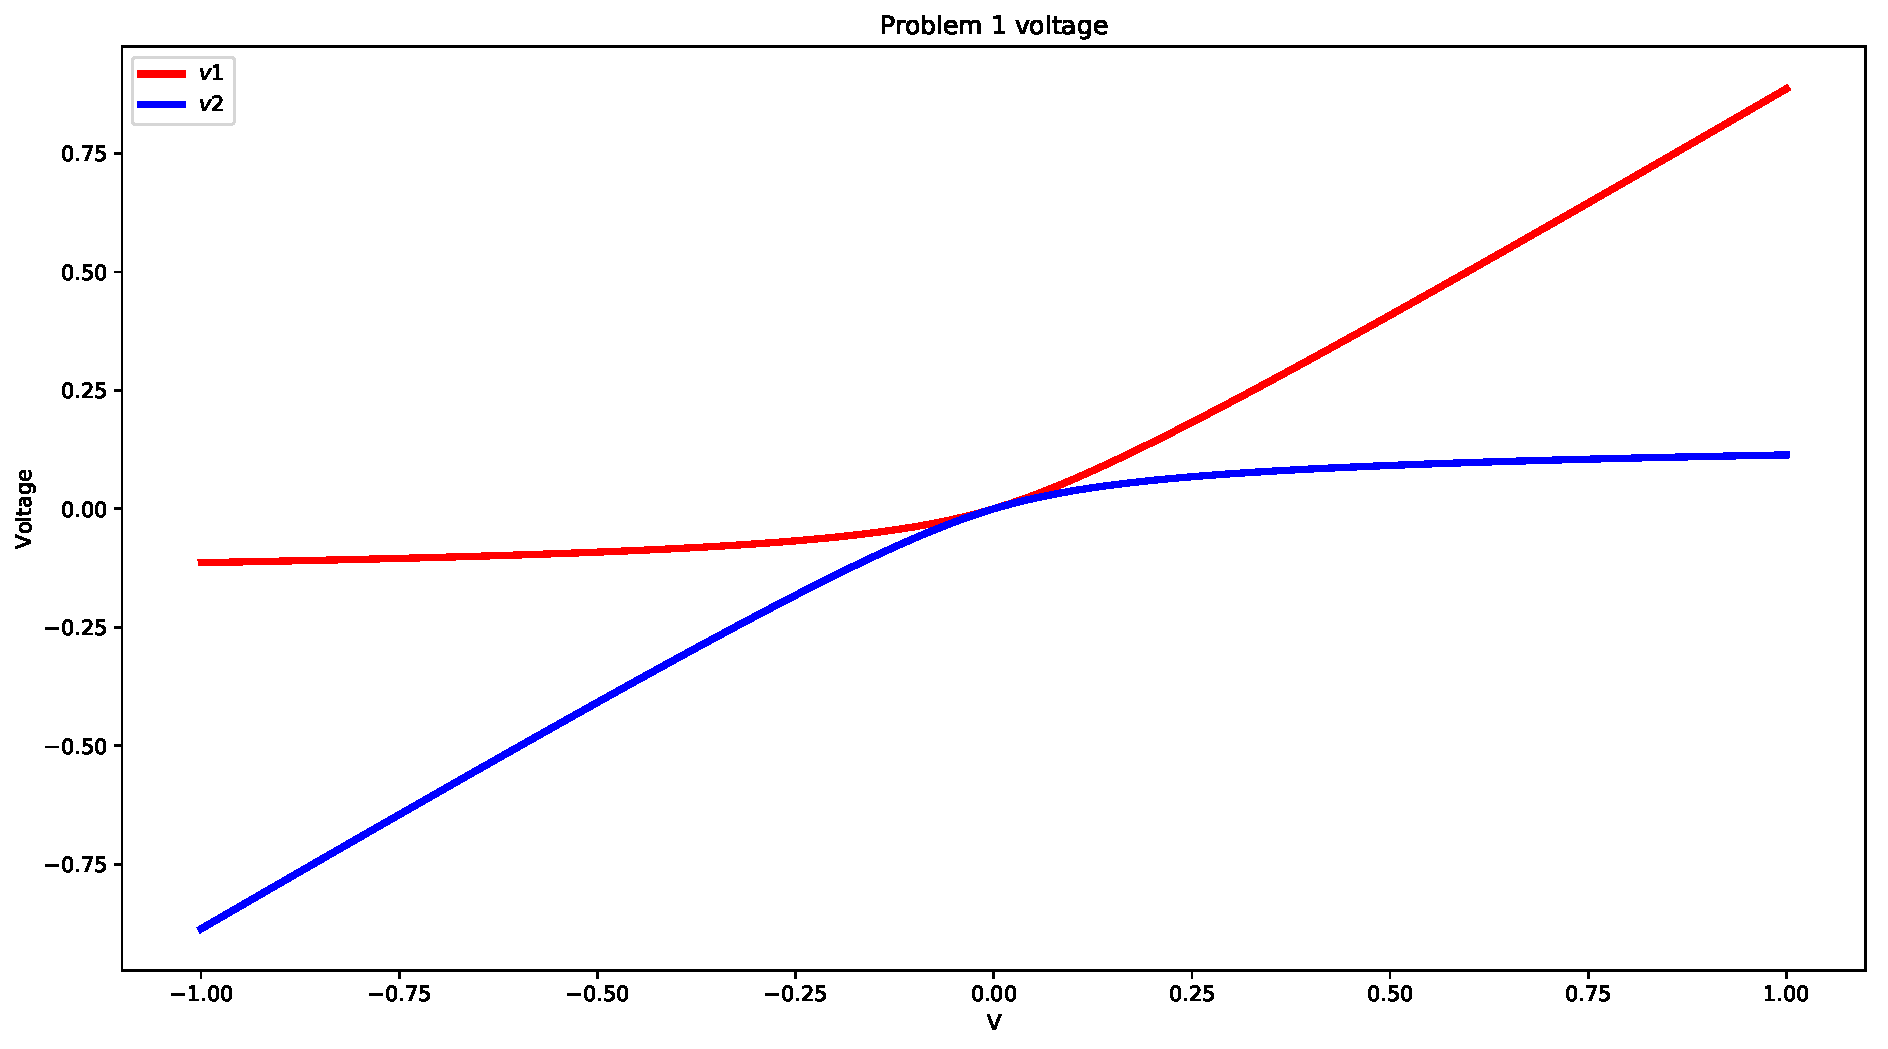
\includegraphics[width=0.8\textwidth]{src/M1_voltage.pdf}
    \caption{Problem 1 result(voltage)}
    \label{fig:M1 volt}
\end{figure}
When V is negative, v1 will be very small and v2 will be close to V, while v1 will be close to V and v2 will be very small when V is positive.
Also, for better upderstanding for this circult, we still need to see the change of current of all diodes as shown in Figure \ref{fig:M1 current}.
\begin{figure}[H]
    \centering
    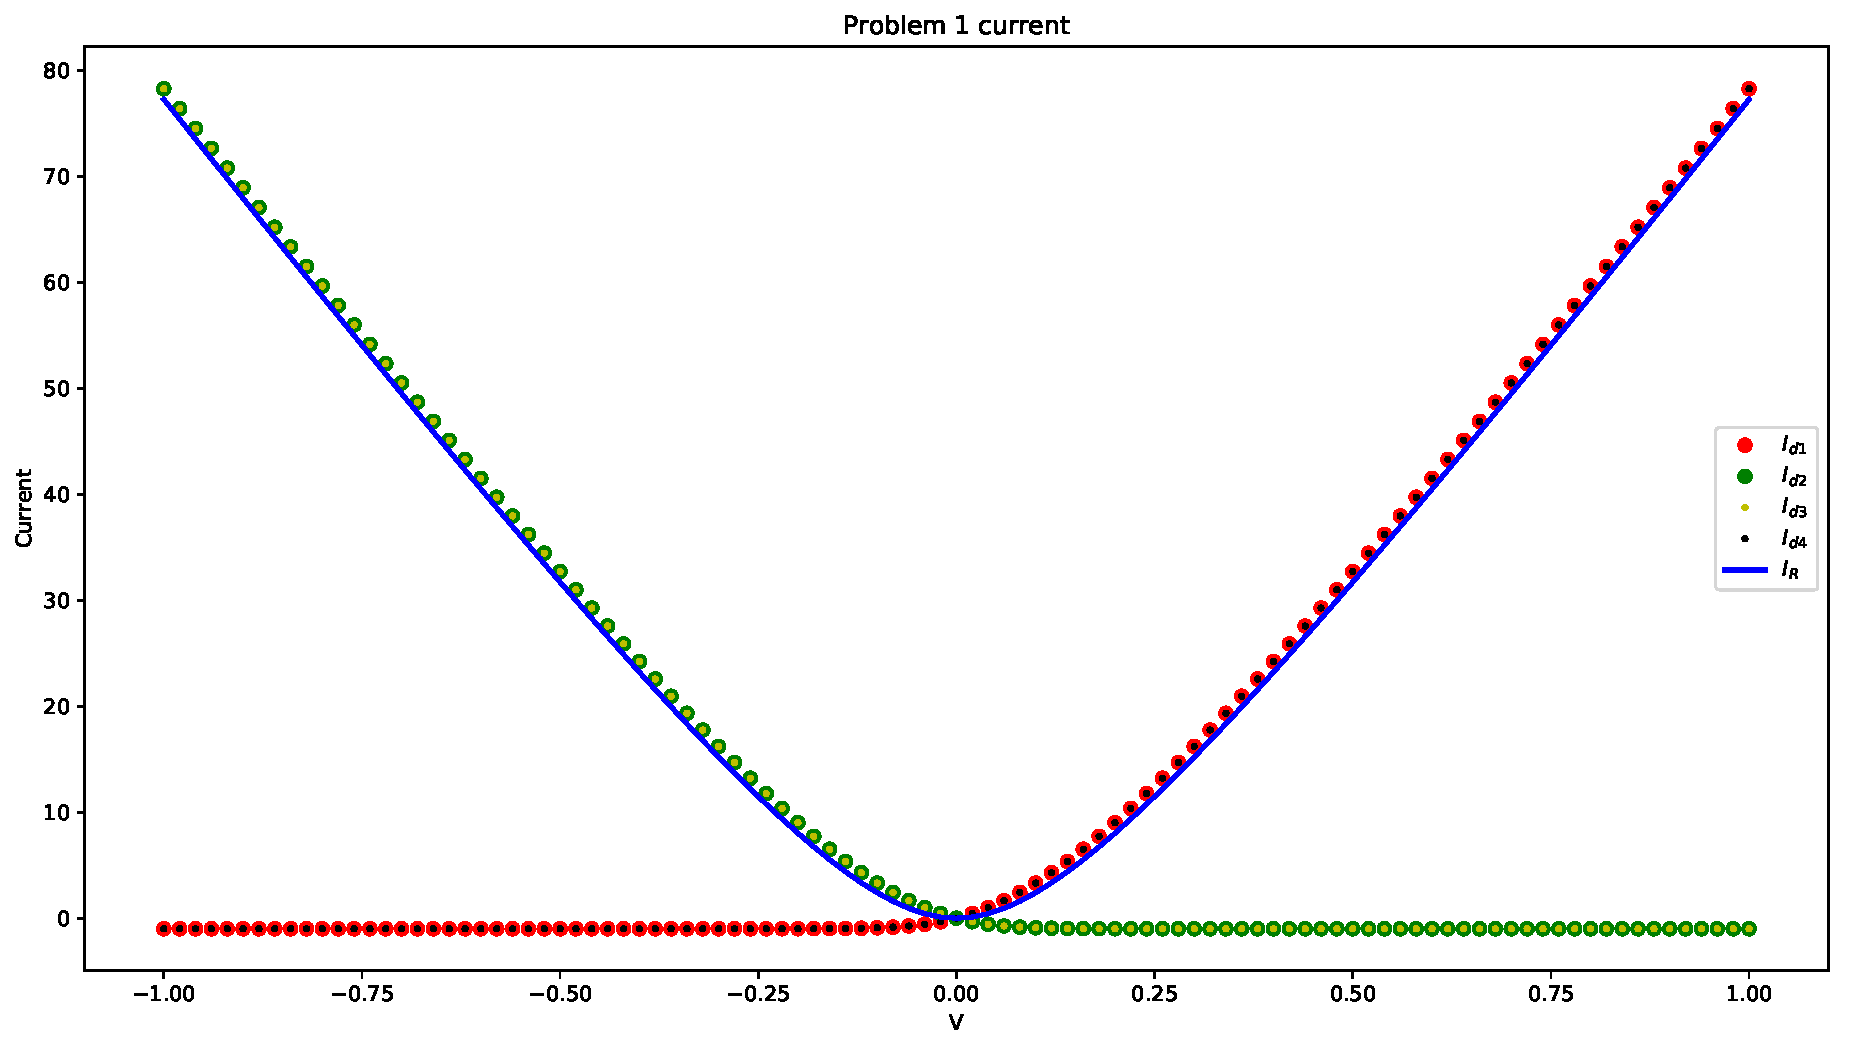
\includegraphics[width=0.8\textwidth]{src/M1_current.pdf}
    \caption{Problem 1 result(current)}
    \label{fig:M1 current}
\end{figure}
From Figure \ref{fig:M1 current}, we can see that $I_{d1}$ and $I_d{4}$ are same and so as $I_{d2}$ and $I_{d3}$. However, $I_R$ is close to 
$I_{d2}$ and $I_{d1}$ when V is negative and positive, respectively.

\subsection{Problem 2}
From Table \ref{tab:problem 1}, we can see the change of $v1$ and $v2$ and current are same as Problem 1 as shown in Figure \ref{fig:M2 volt}
and Figure \ref{fig:M2 current}.
\begin{figure}[H]
    \centering
    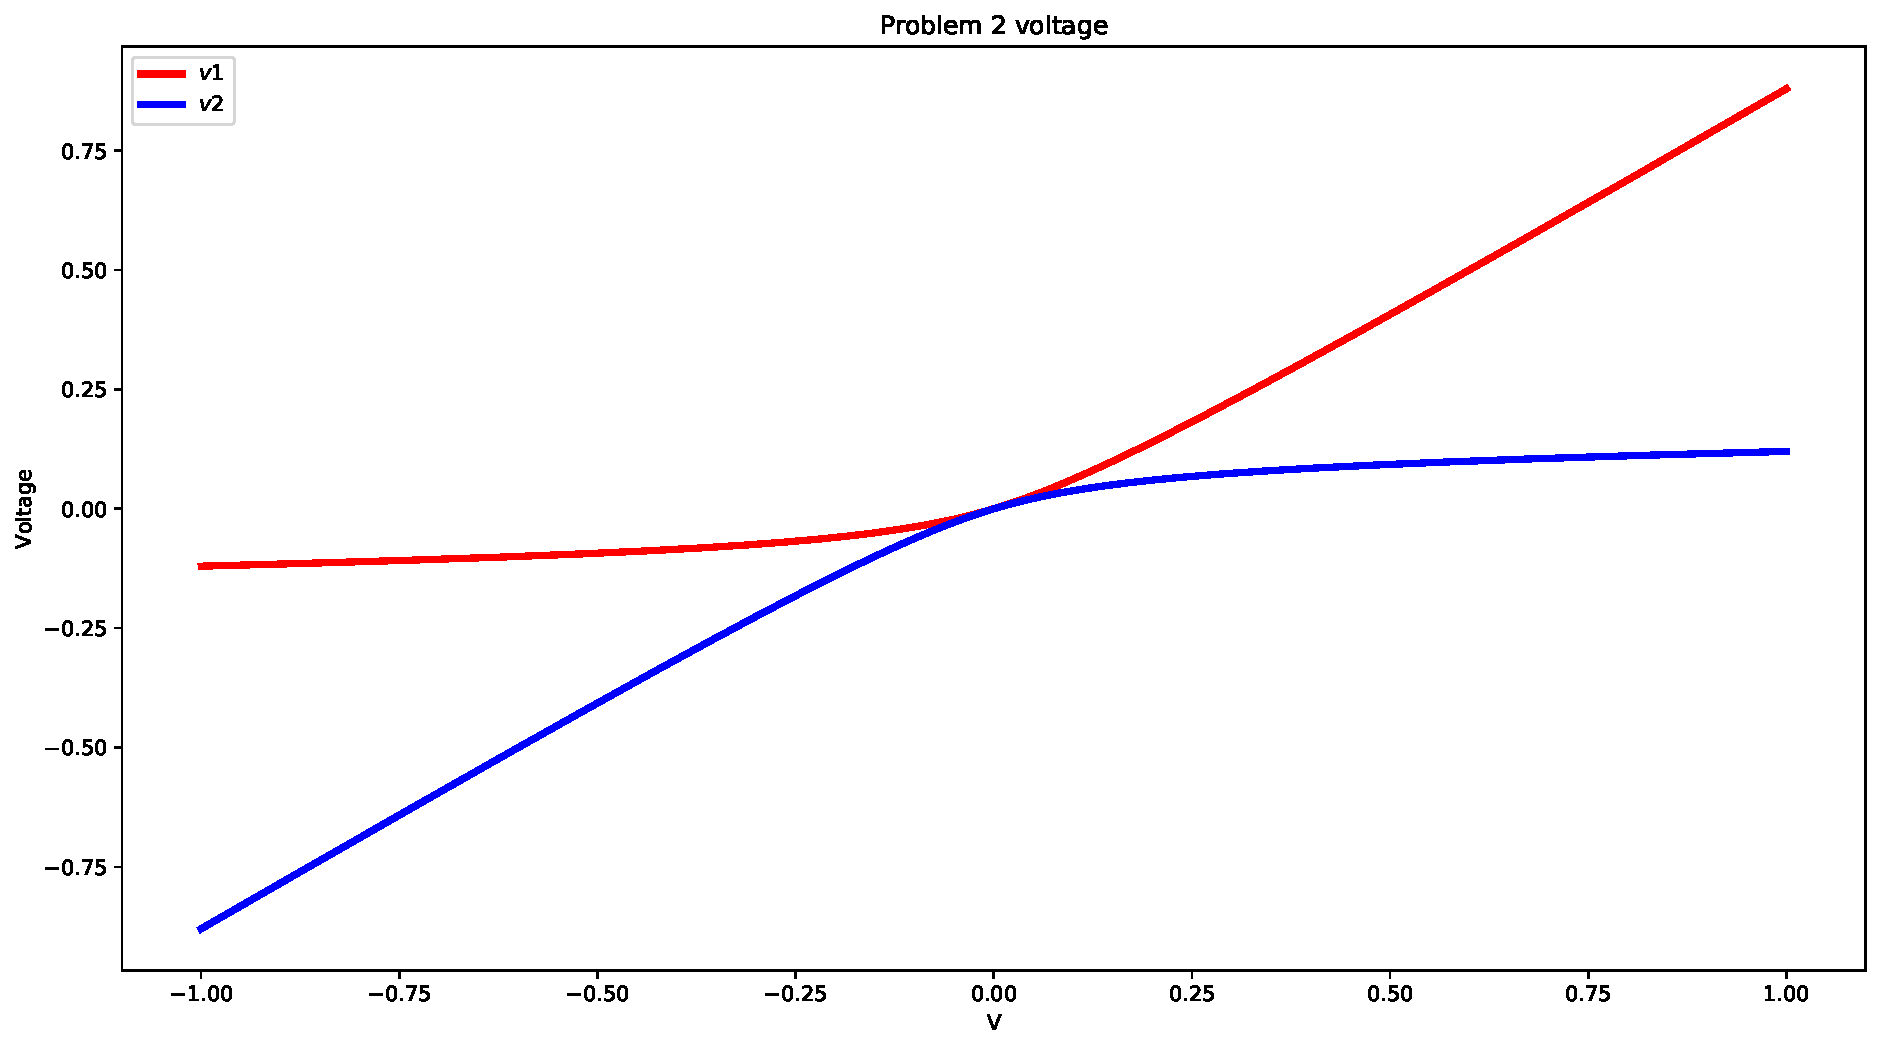
\includegraphics[width=0.8\textwidth]{src/M2_voltage.pdf}
    \caption{Problem 2 result(voltage)}
    \label{fig:M2 volt}
\end{figure}
\begin{figure}[H]
    \centering
    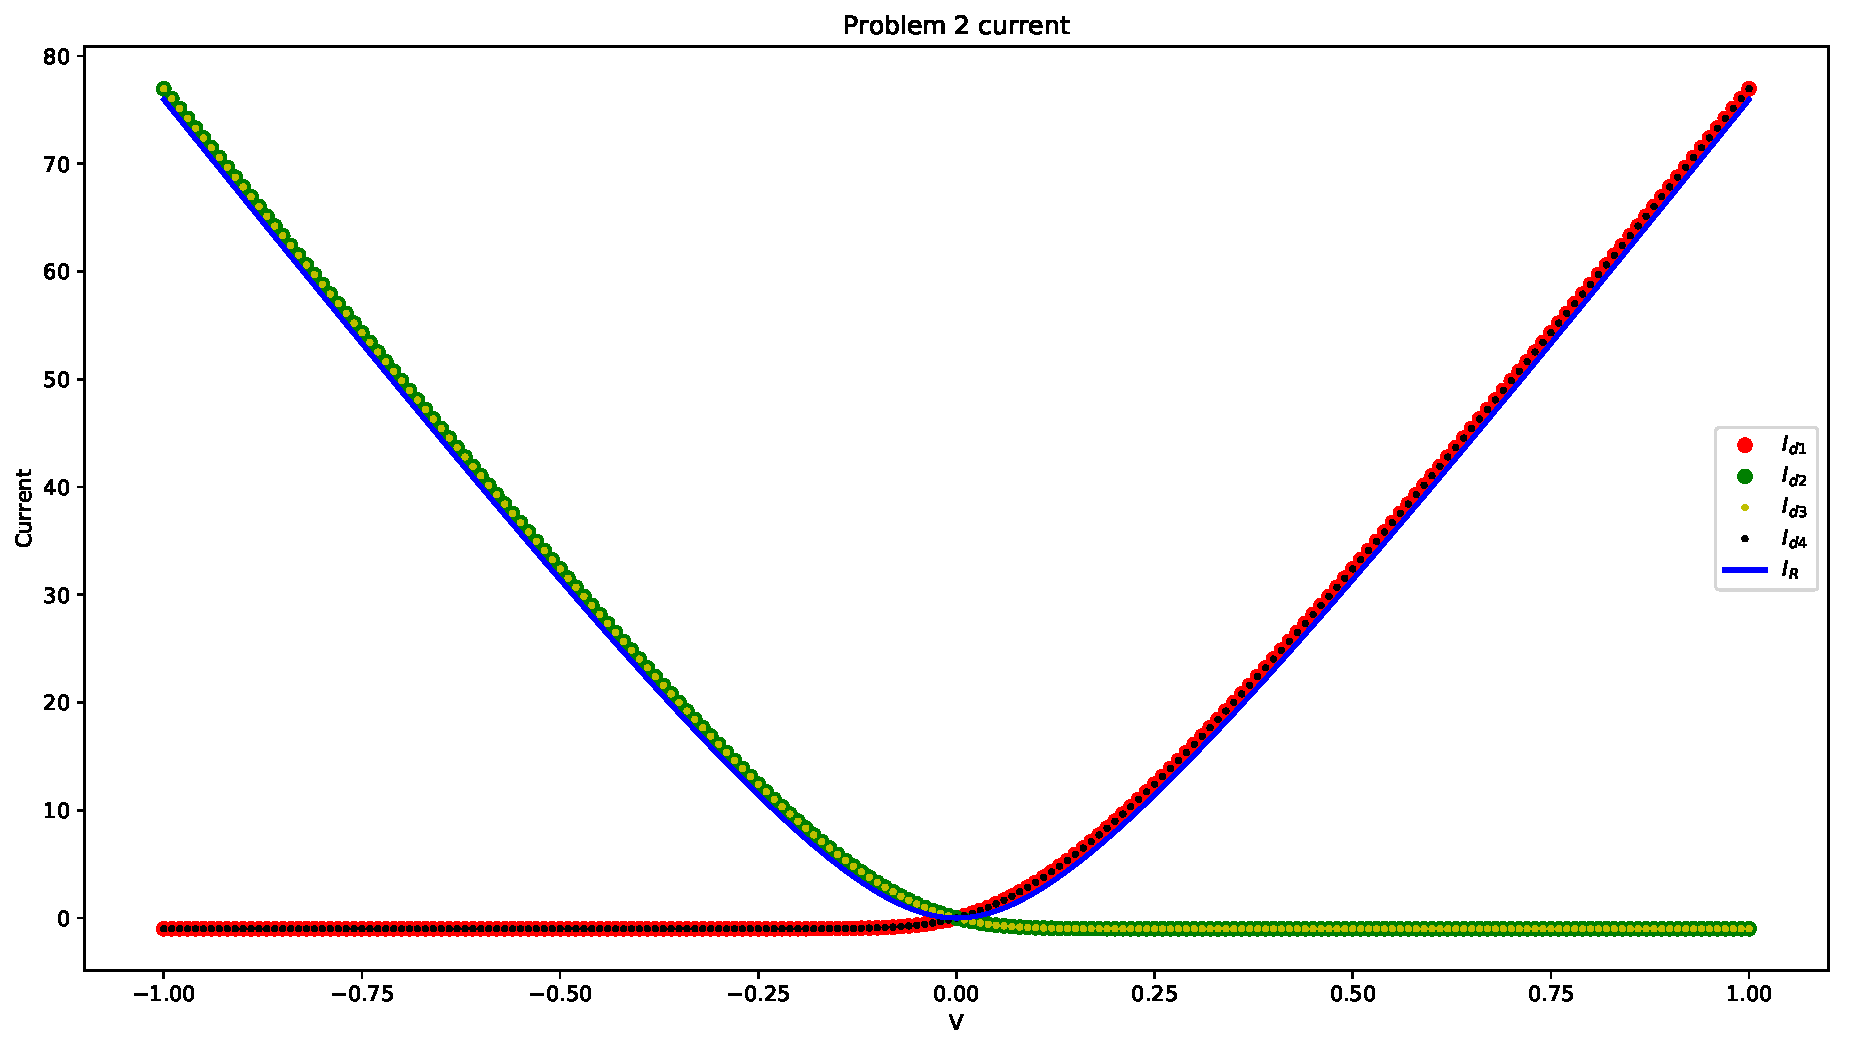
\includegraphics[width=0.8\textwidth]{src/M2_current.pdf}
    \caption{Problem 2 result(current)}
    \label{fig:M2 current}
\end{figure}



\section{Appendix}
\begin{center}
    \begin{longtable}{|c|c|c|c|c|c|c|c|}
    \caption{Problem 1 result} \label{tab:problem 1} \\
        \hline
        V & v1 & v2 & Id1 & Id2 & Id3 & Id4 & Ir \\ \hline
        0 & 0.000E+00 & 0.000E+00 & 0.000E+00 & 0.000E+00 & 0.000E+00 & 0.000E+00 & 0.000E+00 \\ \hline
        0.02 & 1.053E-02 & 9.469E-03 & 4.393E-01 & -3.331E-01 & -3.331E-01 & 4.393E-01 & 1.063E-01 \\ \hline
        0.04 & 2.209E-02 & 1.791E-02 & 9.912E-01 & -5.725E-01 & -5.725E-01 & 9.912E-01 & 4.187E-01 \\ \hline
        0.06 & 3.460E-02 & 2.540E-02 & 1.656E+00 & -7.357E-01 & -7.357E-01 & 1.656E+00 & 9.203E-01 \\ \hline
        0.08 & 4.795E-02 & 3.205E-02 & 2.431E+00 & -8.418E-01 & -8.418E-01 & 2.431E+00 & 1.589E+00 \\ \hline
        0.1 & 6.201E-02 & 3.799E-02 & 3.310E+00 & -9.079E-01 & -9.079E-01 & 3.310E+00 & 2.403E+00 \\ \hline
        0.12 & 7.670E-02 & 4.330E-02 & 4.288E+00 & -9.477E-01 & -9.477E-01 & 4.288E+00 & 3.340E+00 \\ \hline
        0.14 & 9.192E-02 & 4.808E-02 & 5.355E+00 & -9.709E-01 & -9.709E-01 & 5.355E+00 & 4.384E+00 \\ \hline
        0.16 & 1.076E-01 & 5.240E-02 & 6.504E+00 & -9.841E-01 & -9.841E-01 & 6.504E+00 & 5.520E+00 \\ \hline
        0.18 & 1.237E-01 & 5.633E-02 & 7.726E+00 & -9.914E-01 & -9.914E-01 & 7.726E+00 & 6.735E+00 \\ \hline
        0.2 & 1.401E-01 & 5.990E-02 & 9.014E+00 & -9.954E-01 & -9.954E-01 & 9.014E+00 & 8.019E+00 \\ \hline
        0.22 & 1.568E-01 & 6.318E-02 & 1.036E+01 & -9.976E-01 & -9.976E-01 & 1.036E+01 & 9.363E+00 \\ \hline
        0.24 & 1.738E-01 & 6.620E-02 & 1.176E+01 & -9.987E-01 & -9.987E-01 & 1.176E+01 & 1.076E+01 \\ \hline
        0.26 & 1.910E-01 & 6.899E-02 & 1.320E+01 & -9.994E-01 & -9.994E-01 & 1.320E+01 & 1.220E+01 \\ \hline
        0.28 & 2.084E-01 & 7.157E-02 & 1.469E+01 & -9.997E-01 & -9.997E-01 & 1.469E+01 & 1.369E+01 \\ \hline
        0.3 & 2.260E-01 & 7.397E-02 & 1.620E+01 & -9.998E-01 & -9.998E-01 & 1.620E+01 & 1.521E+01 \\ \hline
        0.32 & 2.438E-01 & 7.622E-02 & 1.776E+01 & -9.999E-01 & -9.999E-01 & 1.776E+01 & 1.676E+01 \\ \hline
        0.34 & 2.617E-01 & 7.832E-02 & 1.934E+01 & -1.000E+00 & -1.000E+00 & 1.934E+01 & 1.834E+01 \\ \hline
        0.36 & 2.797E-01 & 8.030E-02 & 2.094E+01 & -1.000E+00 & -1.000E+00 & 2.094E+01 & 1.994E+01 \\ \hline
        0.38 & 2.978E-01 & 8.216E-02 & 2.257E+01 & -1.000E+00 & -1.000E+00 & 2.257E+01 & 2.157E+01 \\ \hline
        0.4 & 3.161E-01 & 8.392E-02 & 2.422E+01 & -1.000E+00 & -1.000E+00 & 2.422E+01 & 2.322E+01 \\ \hline
        0.42 & 3.344E-01 & 8.558E-02 & 2.588E+01 & -1.000E+00 & -1.000E+00 & 2.588E+01 & 2.488E+01 \\ \hline
        0.44 & 3.528E-01 & 8.716E-02 & 2.757E+01 & -1.000E+00 & -1.000E+00 & 2.757E+01 & 2.657E+01 \\ \hline
        0.46 & 3.713E-01 & 8.866E-02 & 2.927E+01 & -1.000E+00 & -1.000E+00 & 2.927E+01 & 2.827E+01 \\ \hline
        0.48 & 3.899E-01 & 9.009E-02 & 3.098E+01 & -1.000E+00 & -1.000E+00 & 3.098E+01 & 2.998E+01 \\ \hline
        0.5 & 4.085E-01 & 9.146E-02 & 3.271E+01 & -1.000E+00 & -1.000E+00 & 3.271E+01 & 3.171E+01 \\ \hline
        0.52 & 4.272E-01 & 9.277E-02 & 3.445E+01 & -1.000E+00 & -1.000E+00 & 3.445E+01 & 3.345E+01 \\ \hline
        0.54 & 4.460E-01 & 9.402E-02 & 3.620E+01 & -1.000E+00 & -1.000E+00 & 3.620E+01 & 3.520E+01 \\ \hline
        0.56 & 4.648E-01 & 9.522E-02 & 3.796E+01 & -1.000E+00 & -1.000E+00 & 3.796E+01 & 3.696E+01 \\ \hline
        0.58 & 4.836E-01 & 9.638E-02 & 3.972E+01 & -1.000E+00 & -1.000E+00 & 3.972E+01 & 3.872E+01 \\ \hline
        0.6 & 5.025E-01 & 9.749E-02 & 4.150E+01 & -1.000E+00 & -1.000E+00 & 4.150E+01 & 4.050E+01 \\ \hline
        0.62 & 5.214E-01 & 9.856E-02 & 4.329E+01 & -1.000E+00 & -1.000E+00 & 4.329E+01 & 4.229E+01 \\ \hline
        0.64 & 5.404E-01 & 9.959E-02 & 4.508E+01 & -1.000E+00 & -1.000E+00 & 4.508E+01 & 4.408E+01 \\ \hline
        0.66 & 5.594E-01 & 1.006E-01 & 4.688E+01 & -1.000E+00 & -1.000E+00 & 4.688E+01 & 4.588E+01 \\ \hline
        0.68 & 5.784E-01 & 1.016E-01 & 4.869E+01 & -1.000E+00 & -1.000E+00 & 4.869E+01 & 4.769E+01 \\ \hline
        0.7 & 5.975E-01 & 1.025E-01 & 5.050E+01 & -1.000E+00 & -1.000E+00 & 5.050E+01 & 4.950E+01 \\ \hline
        0.72 & 6.166E-01 & 1.034E-01 & 5.232E+01 & -1.000E+00 & -1.000E+00 & 5.232E+01 & 5.132E+01 \\ \hline
        0.74 & 6.357E-01 & 1.043E-01 & 5.415E+01 & -1.000E+00 & -1.000E+00 & 5.415E+01 & 5.315E+01 \\ \hline
        0.76 & 6.549E-01 & 1.051E-01 & 5.598E+01 & -1.000E+00 & -1.000E+00 & 5.598E+01 & 5.498E+01 \\ \hline
        0.78 & 6.741E-01 & 1.059E-01 & 5.781E+01 & -1.000E+00 & -1.000E+00 & 5.781E+01 & 5.681E+01 \\ \hline
        0.8 & 6.933E-01 & 1.067E-01 & 5.965E+01 & -1.000E+00 & -1.000E+00 & 5.965E+01 & 5.865E+01 \\ \hline
        0.82 & 7.125E-01 & 1.075E-01 & 6.150E+01 & -1.000E+00 & -1.000E+00 & 6.150E+01 & 6.050E+01 \\ \hline
        0.84 & 7.317E-01 & 1.083E-01 & 6.335E+01 & -1.000E+00 & -1.000E+00 & 6.335E+01 & 6.235E+01 \\ \hline
        0.86 & 7.510E-01 & 1.090E-01 & 6.520E+01 & -1.000E+00 & -1.000E+00 & 6.520E+01 & 6.420E+01 \\ \hline
        0.88 & 7.703E-01 & 1.097E-01 & 6.705E+01 & -1.000E+00 & -1.000E+00 & 6.705E+01 & 6.605E+01 \\ \hline
        0.9 & 7.896E-01 & 1.104E-01 & 6.891E+01 & -1.000E+00 & -1.000E+00 & 6.891E+01 & 6.791E+01 \\ \hline
        0.92 & 8.089E-01 & 1.111E-01 & 7.078E+01 & -1.000E+00 & -1.000E+00 & 7.078E+01 & 6.978E+01 \\ \hline
        0.94 & 8.282E-01 & 1.118E-01 & 7.264E+01 & -1.000E+00 & -1.000E+00 & 7.264E+01 & 7.164E+01 \\ \hline
        0.96 & 8.476E-01 & 1.124E-01 & 7.451E+01 & -1.000E+00 & -1.000E+00 & 7.451E+01 & 7.351E+01 \\ \hline
        0.98 & 8.669E-01 & 1.131E-01 & 7.639E+01 & -1.000E+00 & -1.000E+00 & 7.639E+01 & 7.539E+01 \\ \hline
        1 & 8.863E-01 & 1.137E-01 & 7.826E+01 & -1.000E+00 & -1.000E+00 & 7.826E+01 & 7.726E+01 \\ \hline
        0 & 0.000E+00 & 0.000E+00 & 0.000E+00 & 0.000E+00 & 0.000E+00 & 0.000E+00 & 0.000E+00 \\ \hline
        -0.02 & -9.469E-03 & -1.053E-02 & -3.331E-01 & 4.393E-01 & 4.393E-01 & -3.331E-01 & 1.063E-01 \\ \hline
        -0.04 & -1.791E-02 & -2.209E-02 & -5.725E-01 & 9.912E-01 & 9.912E-01 & -5.725E-01 & 4.187E-01 \\ \hline
        -0.06 & -2.540E-02 & -3.460E-02 & -7.357E-01 & 1.656E+00 & 1.656E+00 & -7.357E-01 & 9.203E-01 \\ \hline
        -0.08 & -3.205E-02 & -4.795E-02 & -8.418E-01 & 2.431E+00 & 2.431E+00 & -8.418E-01 & 1.589E+00 \\ \hline
        -0.1 & -3.799E-02 & -6.201E-02 & -9.079E-01 & 3.310E+00 & 3.310E+00 & -9.079E-01 & 2.403E+00 \\ \hline
        -0.12 & -4.330E-02 & -7.670E-02 & -9.477E-01 & 4.288E+00 & 4.288E+00 & -9.477E-01 & 3.340E+00 \\ \hline
        -0.14 & -4.808E-02 & -9.192E-02 & -9.709E-01 & 5.355E+00 & 5.355E+00 & -9.709E-01 & 4.384E+00 \\ \hline
        -0.16 & -5.240E-02 & -1.076E-01 & -9.841E-01 & 6.504E+00 & 6.504E+00 & -9.841E-01 & 5.520E+00 \\ \hline
        -0.18 & -5.633E-02 & -1.237E-01 & -9.914E-01 & 7.726E+00 & 7.726E+00 & -9.914E-01 & 6.735E+00 \\ \hline
        -0.2 & -5.990E-02 & -1.401E-01 & -9.954E-01 & 9.014E+00 & 9.014E+00 & -9.954E-01 & 8.019E+00 \\ \hline
        -0.22 & -6.318E-02 & -1.568E-01 & -9.976E-01 & 1.036E+01 & 1.036E+01 & -9.976E-01 & 9.363E+00 \\ \hline
        -0.24 & -6.620E-02 & -1.738E-01 & -9.987E-01 & 1.176E+01 & 1.176E+01 & -9.987E-01 & 1.076E+01 \\ \hline
        -0.26 & -6.899E-02 & -1.910E-01 & -9.994E-01 & 1.320E+01 & 1.320E+01 & -9.994E-01 & 1.220E+01 \\ \hline
        -0.28 & -7.157E-02 & -2.084E-01 & -9.997E-01 & 1.469E+01 & 1.469E+01 & -9.997E-01 & 1.369E+01 \\ \hline
        -0.3 & -7.397E-02 & -2.260E-01 & -9.998E-01 & 1.620E+01 & 1.620E+01 & -9.998E-01 & 1.521E+01 \\ \hline
        -0.32 & -7.622E-02 & -2.438E-01 & -9.999E-01 & 1.776E+01 & 1.776E+01 & -9.999E-01 & 1.676E+01 \\ \hline
        -0.34 & -7.832E-02 & -2.617E-01 & -1.000E+00 & 1.934E+01 & 1.934E+01 & -1.000E+00 & 1.834E+01 \\ \hline
        -0.36 & -8.030E-02 & -2.797E-01 & -1.000E+00 & 2.094E+01 & 2.094E+01 & -1.000E+00 & 1.994E+01 \\ \hline
        -0.38 & -8.216E-02 & -2.978E-01 & -1.000E+00 & 2.257E+01 & 2.257E+01 & -1.000E+00 & 2.157E+01 \\ \hline
        -0.4 & -8.392E-02 & -3.161E-01 & -1.000E+00 & 2.422E+01 & 2.422E+01 & -1.000E+00 & 2.322E+01 \\ \hline
        -0.42 & -8.558E-02 & -3.344E-01 & -1.000E+00 & 2.588E+01 & 2.588E+01 & -1.000E+00 & 2.488E+01 \\ \hline
        -0.44 & -8.716E-02 & -3.528E-01 & -1.000E+00 & 2.757E+01 & 2.757E+01 & -1.000E+00 & 2.657E+01 \\ \hline
        -0.46 & -8.866E-02 & -3.713E-01 & -1.000E+00 & 2.927E+01 & 2.927E+01 & -1.000E+00 & 2.827E+01 \\ \hline
        -0.48 & -9.009E-02 & -3.899E-01 & -1.000E+00 & 3.098E+01 & 3.098E+01 & -1.000E+00 & 2.998E+01 \\ \hline
        -0.5 & -9.146E-02 & -4.085E-01 & -1.000E+00 & 3.271E+01 & 3.271E+01 & -1.000E+00 & 3.171E+01 \\ \hline
        -0.52 & -9.277E-02 & -4.272E-01 & -1.000E+00 & 3.445E+01 & 3.445E+01 & -1.000E+00 & 3.345E+01 \\ \hline
        -0.54 & -9.402E-02 & -4.460E-01 & -1.000E+00 & 3.620E+01 & 3.620E+01 & -1.000E+00 & 3.520E+01 \\ \hline
        -0.56 & -9.522E-02 & -4.648E-01 & -1.000E+00 & 3.796E+01 & 3.796E+01 & -1.000E+00 & 3.696E+01 \\ \hline
        -0.58 & -9.638E-02 & -4.836E-01 & -1.000E+00 & 3.972E+01 & 3.972E+01 & -1.000E+00 & 3.872E+01 \\ \hline
        -0.6 & -9.749E-02 & -5.025E-01 & -1.000E+00 & 4.150E+01 & 4.150E+01 & -1.000E+00 & 4.050E+01 \\ \hline
        -0.62 & -9.856E-02 & -5.214E-01 & -1.000E+00 & 4.329E+01 & 4.329E+01 & -1.000E+00 & 4.229E+01 \\ \hline
        -0.64 & -9.959E-02 & -5.404E-01 & -1.000E+00 & 4.508E+01 & 4.508E+01 & -1.000E+00 & 4.408E+01 \\ \hline
        -0.66 & -1.006E-01 & -5.594E-01 & -1.000E+00 & 4.688E+01 & 4.688E+01 & -1.000E+00 & 4.588E+01 \\ \hline
        -0.68 & -1.016E-01 & -5.784E-01 & -1.000E+00 & 4.869E+01 & 4.869E+01 & -1.000E+00 & 4.769E+01 \\ \hline
        -0.7 & -1.025E-01 & -5.975E-01 & -1.000E+00 & 5.050E+01 & 5.050E+01 & -1.000E+00 & 4.950E+01 \\ \hline
        -0.72 & -1.034E-01 & -6.166E-01 & -1.000E+00 & 5.232E+01 & 5.232E+01 & -1.000E+00 & 5.132E+01 \\ \hline
        -0.74 & -1.043E-01 & -6.357E-01 & -1.000E+00 & 5.415E+01 & 5.415E+01 & -1.000E+00 & 5.315E+01 \\ \hline
        -0.76 & -1.051E-01 & -6.549E-01 & -1.000E+00 & 5.598E+01 & 5.598E+01 & -1.000E+00 & 5.498E+01 \\ \hline
        -0.78 & -1.059E-01 & -6.741E-01 & -1.000E+00 & 5.781E+01 & 5.781E+01 & -1.000E+00 & 5.681E+01 \\ \hline
        -0.8 & -1.067E-01 & -6.933E-01 & -1.000E+00 & 5.965E+01 & 5.965E+01 & -1.000E+00 & 5.865E+01 \\ \hline
        -0.82 & -1.075E-01 & -7.125E-01 & -1.000E+00 & 6.150E+01 & 6.150E+01 & -1.000E+00 & 6.050E+01 \\ \hline
        -0.84 & -1.083E-01 & -7.317E-01 & -1.000E+00 & 6.335E+01 & 6.335E+01 & -1.000E+00 & 6.235E+01 \\ \hline
        -0.86 & -1.090E-01 & -7.510E-01 & -1.000E+00 & 6.520E+01 & 6.520E+01 & -1.000E+00 & 6.420E+01 \\ \hline
        -0.88 & -1.097E-01 & -7.703E-01 & -1.000E+00 & 6.705E+01 & 6.705E+01 & -1.000E+00 & 6.605E+01 \\ \hline
        -0.9 & -1.104E-01 & -7.896E-01 & -1.000E+00 & 6.891E+01 & 6.891E+01 & -1.000E+00 & 6.791E+01 \\ \hline
        -0.92 & -1.111E-01 & -8.089E-01 & -1.000E+00 & 7.078E+01 & 7.078E+01 & -1.000E+00 & 6.978E+01 \\ \hline
        -0.94 & -1.118E-01 & -8.282E-01 & -1.000E+00 & 7.264E+01 & 7.264E+01 & -1.000E+00 & 7.164E+01 \\ \hline
        -0.96 & -1.124E-01 & -8.476E-01 & -1.000E+00 & 7.451E+01 & 7.451E+01 & -1.000E+00 & 7.351E+01 \\ \hline
        -0.98 & -1.131E-01 & -8.669E-01 & -1.000E+00 & 7.639E+01 & 7.639E+01 & -1.000E+00 & 7.539E+01 \\ \hline
        -1 & -1.137E-01 & -8.863E-01 & -1.000E+00 & 7.826E+01 & 7.826E+01 & -1.000E+00 & 7.726E+01 \\ \hline
    \end{longtable}
\end{center}

\begin{center}
    \begin{longtable}{|c|c|c|c|c|c|c|c|}
        \caption{Problem 2 result(voltage and current)} \label{tab:problem 2 volt} \\
    \hline
    V & v1 & v2 & Id1 & Id2 & Id3 & Id4 & Ir \\ \hline
    0 & 0.000E+00 & 0.000E+00 & 0.000E+00 & 0.000E+00 & 0.000E+00 & 0.000E+00 & 0.000E+00 \\ \hline
    0.01 & 5.133E-03 & 4.867E-03 & 2.058E-01 & -1.792E-01 & -1.792E-01 & 2.058E-01 & 2.667E-02 \\ \hline
    0.02 & 1.053E-02 & 9.469E-03 & 4.393E-01 & -3.331E-01 & -3.331E-01 & 4.393E-01 & 1.063E-01 \\ \hline
    0.03 & 1.619E-02 & 1.381E-02 & 7.010E-01 & -4.634E-01 & -4.634E-01 & 7.010E-01 & 2.375E-01 \\ \hline
    0.04 & 2.209E-02 & 1.791E-02 & 9.910E-01 & -5.724E-01 & -5.724E-01 & 9.910E-01 & 4.186E-01 \\ \hline
    0.05 & 2.823E-02 & 2.177E-02 & 1.309E+00 & -6.624E-01 & -6.624E-01 & 1.309E+00 & 6.470E-01 \\ \hline
    0.06 & 3.460E-02 & 2.540E-02 & 1.656E+00 & -7.357E-01 & -7.357E-01 & 1.656E+00 & 9.199E-01 \\ \hline
    0.07 & 4.117E-02 & 2.883E-02 & 2.029E+00 & -7.947E-01 & -7.947E-01 & 2.029E+00 & 1.235E+00 \\ \hline
    0.08 & 4.794E-02 & 3.206E-02 & 2.430E+00 & -8.417E-01 & -8.417E-01 & 2.430E+00 & 1.588E+00 \\ \hline
    0.09 & 5.489E-02 & 3.511E-02 & 2.856E+00 & -8.788E-01 & -8.788E-01 & 2.856E+00 & 1.977E+00 \\ \hline
    0.1 & 6.200E-02 & 3.800E-02 & 3.308E+00 & -9.078E-01 & -9.078E-01 & 3.308E+00 & 2.400E+00 \\ \hline
    0.11 & 6.927E-02 & 4.073E-02 & 3.783E+00 & -9.303E-01 & -9.303E-01 & 3.783E+00 & 2.853E+00 \\ \hline
    0.12 & 7.667E-02 & 4.333E-02 & 4.282E+00 & -9.475E-01 & -9.475E-01 & 4.282E+00 & 3.335E+00 \\ \hline
    0.13 & 8.421E-02 & 4.579E-02 & 4.803E+00 & -9.607E-01 & -9.607E-01 & 4.803E+00 & 3.843E+00 \\ \hline
    0.14 & 9.188E-02 & 4.812E-02 & 5.346E+00 & -9.707E-01 & -9.707E-01 & 5.346E+00 & 4.375E+00 \\ \hline
    0.15 & 9.965E-02 & 5.035E-02 & 5.908E+00 & -9.783E-01 & -9.783E-01 & 5.908E+00 & 4.930E+00 \\ \hline
    0.16 & 1.075E-01 & 5.247E-02 & 6.490E+00 & -9.840E-01 & -9.840E-01 & 6.490E+00 & 5.506E+00 \\ \hline
    0.17 & 1.155E-01 & 5.449E-02 & 7.089E+00 & -9.882E-01 & -9.882E-01 & 7.089E+00 & 6.101E+00 \\ \hline
    0.18 & 1.236E-01 & 5.643E-02 & 7.706E+00 & -9.913E-01 & -9.913E-01 & 7.706E+00 & 6.715E+00 \\ \hline
    0.19 & 1.317E-01 & 5.828E-02 & 8.338E+00 & -9.937E-01 & -9.937E-01 & 8.338E+00 & 7.345E+00 \\ \hline
    0.2 & 1.400E-01 & 6.005E-02 & 8.986E+00 & -9.954E-01 & -9.954E-01 & 8.986E+00 & 7.991E+00 \\ \hline
    0.21 & 1.483E-01 & 6.174E-02 & 9.648E+00 & -9.966E-01 & -9.966E-01 & 9.648E+00 & 8.651E+00 \\ \hline
    0.22 & 1.566E-01 & 6.337E-02 & 1.032E+01 & -9.976E-01 & -9.976E-01 & 1.032E+01 & 9.325E+00 \\ \hline
    0.23 & 1.651E-01 & 6.494E-02 & 1.101E+01 & -9.982E-01 & -9.982E-01 & 1.101E+01 & 1.001E+01 \\ \hline
    0.24 & 1.736E-01 & 6.644E-02 & 1.171E+01 & -9.987E-01 & -9.987E-01 & 1.171E+01 & 1.071E+01 \\ \hline
    0.25 & 1.821E-01 & 6.790E-02 & 1.242E+01 & -9.991E-01 & -9.991E-01 & 1.242E+01 & 1.142E+01 \\ \hline
    0.26 & 1.907E-01 & 6.929E-02 & 1.314E+01 & -9.993E-01 & -9.993E-01 & 1.314E+01 & 1.214E+01 \\ \hline
    0.27 & 1.994E-01 & 7.064E-02 & 1.387E+01 & -9.995E-01 & -9.995E-01 & 1.387E+01 & 1.287E+01 \\ \hline
    0.28 & 2.081E-01 & 7.195E-02 & 1.461E+01 & -9.997E-01 & -9.997E-01 & 1.461E+01 & 1.361E+01 \\ \hline
    0.29 & 2.168E-01 & 7.321E-02 & 1.536E+01 & -9.998E-01 & -9.998E-01 & 1.536E+01 & 1.436E+01 \\ \hline
    0.3 & 2.256E-01 & 7.443E-02 & 1.611E+01 & -9.998E-01 & -9.998E-01 & 1.611E+01 & 1.511E+01 \\ \hline
    0.31 & 2.344E-01 & 7.561E-02 & 1.688E+01 & -9.999E-01 & -9.999E-01 & 1.688E+01 & 1.588E+01 \\ \hline
    0.32 & 2.432E-01 & 7.676E-02 & 1.765E+01 & -9.999E-01 & -9.999E-01 & 1.765E+01 & 1.665E+01 \\ \hline
    0.33 & 2.521E-01 & 7.787E-02 & 1.843E+01 & -9.999E-01 & -9.999E-01 & 1.843E+01 & 1.743E+01 \\ \hline
    0.34 & 2.610E-01 & 7.895E-02 & 1.921E+01 & -1.000E+00 & -1.000E+00 & 1.921E+01 & 1.821E+01 \\ \hline
    0.35 & 2.700E-01 & 8.000E-02 & 2.000E+01 & -1.000E+00 & -1.000E+00 & 2.000E+01 & 1.900E+01 \\ \hline
    0.36 & 2.790E-01 & 8.102E-02 & 2.080E+01 & -1.000E+00 & -1.000E+00 & 2.080E+01 & 1.980E+01 \\ \hline
    0.37 & 2.880E-01 & 8.202E-02 & 2.160E+01 & -1.000E+00 & -1.000E+00 & 2.160E+01 & 2.060E+01 \\ \hline
    0.38 & 2.970E-01 & 8.299E-02 & 2.240E+01 & -1.000E+00 & -1.000E+00 & 2.240E+01 & 2.140E+01 \\ \hline
    0.39 & 3.061E-01 & 8.394E-02 & 2.321E+01 & -1.000E+00 & -1.000E+00 & 2.321E+01 & 2.221E+01 \\ \hline
    0.4 & 3.151E-01 & 8.486E-02 & 2.403E+01 & -1.000E+00 & -1.000E+00 & 2.403E+01 & 2.303E+01 \\ \hline
    0.41 & 3.242E-01 & 8.576E-02 & 2.485E+01 & -1.000E+00 & -1.000E+00 & 2.485E+01 & 2.385E+01 \\ \hline
    0.42 & 3.334E-01 & 8.664E-02 & 2.567E+01 & -1.000E+00 & -1.000E+00 & 2.567E+01 & 2.467E+01 \\ \hline
    0.43 & 3.425E-01 & 8.750E-02 & 2.650E+01 & -1.000E+00 & -1.000E+00 & 2.650E+01 & 2.550E+01 \\ \hline
    0.44 & 3.517E-01 & 8.834E-02 & 2.733E+01 & -1.000E+00 & -1.000E+00 & 2.733E+01 & 2.633E+01 \\ \hline
    0.45 & 3.608E-01 & 8.917E-02 & 2.817E+01 & -1.000E+00 & -1.000E+00 & 2.817E+01 & 2.717E+01 \\ \hline
    0.46 & 3.700E-01 & 8.997E-02 & 2.901E+01 & -1.000E+00 & -1.000E+00 & 2.901E+01 & 2.801E+01 \\ \hline
    0.47 & 3.792E-01 & 9.077E-02 & 2.985E+01 & -1.000E+00 & -1.000E+00 & 2.985E+01 & 2.885E+01 \\ \hline
    0.48 & 3.885E-01 & 9.154E-02 & 3.069E+01 & -1.000E+00 & -1.000E+00 & 3.069E+01 & 2.969E+01 \\ \hline
    0.49 & 3.977E-01 & 9.230E-02 & 3.154E+01 & -1.000E+00 & -1.000E+00 & 3.154E+01 & 3.054E+01 \\ \hline
    0.5 & 4.070E-01 & 9.305E-02 & 3.239E+01 & -1.000E+00 & -1.000E+00 & 3.239E+01 & 3.139E+01 \\ \hline
    0.51 & 4.162E-01 & 9.378E-02 & 3.324E+01 & -1.000E+00 & -1.000E+00 & 3.324E+01 & 3.224E+01 \\ \hline
    0.52 & 4.255E-01 & 9.450E-02 & 3.410E+01 & -1.000E+00 & -1.000E+00 & 3.410E+01 & 3.310E+01 \\ \hline
    0.53 & 4.348E-01 & 9.521E-02 & 3.496E+01 & -1.000E+00 & -1.000E+00 & 3.496E+01 & 3.396E+01 \\ \hline
    0.54 & 4.441E-01 & 9.590E-02 & 3.582E+01 & -1.000E+00 & -1.000E+00 & 3.582E+01 & 3.482E+01 \\ \hline
    0.55 & 4.534E-01 & 9.659E-02 & 3.668E+01 & -1.000E+00 & -1.000E+00 & 3.668E+01 & 3.568E+01 \\ \hline
    0.56 & 4.627E-01 & 9.726E-02 & 3.755E+01 & -1.000E+00 & -1.000E+00 & 3.755E+01 & 3.655E+01 \\ \hline
    0.57 & 4.721E-01 & 9.792E-02 & 3.842E+01 & -1.000E+00 & -1.000E+00 & 3.842E+01 & 3.742E+01 \\ \hline
0.58 & 4.814E-01 & 9.858E-02 & 3.928E+01 & -1.000E+00 & -1.000E+00 & 3.928E+01 & 3.828E+01 \\ \hline
0.59 & 4.908E-01 & 9.922E-02 & 4.016E+01 & -1.000E+00 & -1.000E+00 & 4.016E+01 & 3.916E+01 \\ \hline
0.6 & 5.001E-01 & 9.985E-02 & 4.103E+01 & -1.000E+00 & -1.000E+00 & 4.103E+01 & 4.003E+01 \\ \hline
0.61 & 5.095E-01 & 1.005E-01 & 4.190E+01 & -1.000E+00 & -1.000E+00 & 4.190E+01 & 4.090E+01 \\ \hline
0.62 & 5.189E-01 & 1.011E-01 & 4.278E+01 & -1.000E+00 & -1.000E+00 & 4.278E+01 & 4.178E+01 \\ \hline
0.63 & 5.283E-01 & 1.017E-01 & 4.366E+01 & -1.000E+00 & -1.000E+00 & 4.366E+01 & 4.266E+01 \\ \hline
0.64 & 5.377E-01 & 1.023E-01 & 4.454E+01 & -1.000E+00 & -1.000E+00 & 4.454E+01 & 4.354E+01 \\ \hline
0.65 & 5.471E-01 & 1.029E-01 & 4.542E+01 & -1.000E+00 & -1.000E+00 & 4.542E+01 & 4.442E+01 \\ \hline
0.66 & 5.565E-01 & 1.035E-01 & 4.631E+01 & -1.000E+00 & -1.000E+00 & 4.631E+01 & 4.531E+01 \\ \hline
0.67 & 5.659E-01 & 1.041E-01 & 4.719E+01 & -1.000E+00 & -1.000E+00 & 4.719E+01 & 4.619E+01 \\ \hline
0.68 & 5.754E-01 & 1.046E-01 & 4.808E+01 & -1.000E+00 & -1.000E+00 & 4.808E+01 & 4.708E+01 \\ \hline
0.69 & 5.848E-01 & 1.052E-01 & 4.896E+01 & -1.000E+00 & -1.000E+00 & 4.896E+01 & 4.796E+01 \\ \hline
0.7 & 5.943E-01 & 1.057E-01 & 4.985E+01 & -1.000E+00 & -1.000E+00 & 4.985E+01 & 4.885E+01 \\ \hline
0.71 & 6.037E-01 & 1.063E-01 & 5.074E+01 & -1.000E+00 & -1.000E+00 & 5.074E+01 & 4.974E+01 \\ \hline
0.72 & 6.132E-01 & 1.068E-01 & 5.163E+01 & -1.000E+00 & -1.000E+00 & 5.163E+01 & 5.063E+01 \\ \hline
0.73 & 6.226E-01 & 1.074E-01 & 5.253E+01 & -1.000E+00 & -1.000E+00 & 5.253E+01 & 5.153E+01 \\ \hline
0.74 & 6.321E-01 & 1.079E-01 & 5.342E+01 & -1.000E+00 & -1.000E+00 & 5.342E+01 & 5.242E+01 \\ \hline
0.75 & 6.416E-01 & 1.084E-01 & 5.431E+01 & -1.000E+00 & -1.000E+00 & 5.431E+01 & 5.331E+01 \\ \hline
0.76 & 6.510E-01 & 1.090E-01 & 5.521E+01 & -1.000E+00 & -1.000E+00 & 5.521E+01 & 5.421E+01 \\ \hline
0.77 & 6.605E-01 & 1.095E-01 & 5.611E+01 & -1.000E+00 & -1.000E+00 & 5.611E+01 & 5.511E+01 \\ \hline
0.78 & 6.700E-01 & 1.100E-01 & 5.700E+01 & -1.000E+00 & -1.000E+00 & 5.700E+01 & 5.600E+01 \\ \hline
0.79 & 6.795E-01 & 1.105E-01 & 5.790E+01 & -1.000E+00 & -1.000E+00 & 5.790E+01 & 5.690E+01 \\ \hline
0.8 & 6.890E-01 & 1.110E-01 & 5.880E+01 & -1.000E+00 & -1.000E+00 & 5.880E+01 & 5.780E+01 \\ \hline
0.81 & 6.985E-01 & 1.115E-01 & 5.970E+01 & -1.000E+00 & -1.000E+00 & 5.970E+01 & 5.870E+01 \\ \hline
0.82 & 7.080E-01 & 1.120E-01 & 6.060E+01 & -1.000E+00 & -1.000E+00 & 6.060E+01 & 5.960E+01 \\ \hline
0.83 & 7.175E-01 & 1.125E-01 & 6.151E+01 & -1.000E+00 & -1.000E+00 & 6.151E+01 & 6.051E+01 \\ \hline
0.84 & 7.270E-01 & 1.130E-01 & 6.241E+01 & -1.000E+00 & -1.000E+00 & 6.241E+01 & 6.141E+01 \\ \hline
0.85 & 7.366E-01 & 1.134E-01 & 6.331E+01 & -1.000E+00 & -1.000E+00 & 6.331E+01 & 6.231E+01 \\ \hline
0.86 & 7.461E-01 & 1.139E-01 & 6.422E+01 & -1.000E+00 & -1.000E+00 & 6.422E+01 & 6.322E+01 \\ \hline
0.87 & 7.556E-01 & 1.144E-01 & 6.512E+01 & -1.000E+00 & -1.000E+00 & 6.512E+01 & 6.412E+01 \\ \hline
0.88 & 7.651E-01 & 1.149E-01 & 6.603E+01 & -1.000E+00 & -1.000E+00 & 6.603E+01 & 6.503E+01 \\ \hline
0.89 & 7.747E-01 & 1.153E-01 & 6.693E+01 & -1.000E+00 & -1.000E+00 & 6.693E+01 & 6.593E+01 \\ \hline
0.9 & 7.842E-01 & 1.158E-01 & 6.784E+01 & -1.000E+00 & -1.000E+00 & 6.784E+01 & 6.684E+01 \\ \hline
0.91 & 7.938E-01 & 1.162E-01 & 6.875E+01 & -1.000E+00 & -1.000E+00 & 6.875E+01 & 6.775E+01 \\ \hline
0.92 & 8.033E-01 & 1.167E-01 & 6.966E+01 & -1.000E+00 & -1.000E+00 & 6.966E+01 & 6.866E+01 \\ \hline
0.93 & 8.128E-01 & 1.172E-01 & 7.057E+01 & -1.000E+00 & -1.000E+00 & 7.057E+01 & 6.957E+01 \\ \hline
0.94 & 8.224E-01 & 1.176E-01 & 7.148E+01 & -1.000E+00 & -1.000E+00 & 7.148E+01 & 7.048E+01 \\ \hline
0.95 & 8.319E-01 & 1.181E-01 & 7.239E+01 & -1.000E+00 & -1.000E+00 & 7.239E+01 & 7.139E+01 \\ \hline
0.96 & 8.415E-01 & 1.185E-01 & 7.330E+01 & -1.000E+00 & -1.000E+00 & 7.330E+01 & 7.230E+01 \\ \hline
0.97 & 8.511E-01 & 1.189E-01 & 7.421E+01 & -1.000E+00 & -1.000E+00 & 7.421E+01 & 7.321E+01 \\ \hline
0.98 & 8.606E-01 & 1.194E-01 & 7.512E+01 & -1.000E+00 & -1.000E+00 & 7.512E+01 & 7.412E+01 \\ \hline
0.99 & 8.702E-01 & 1.198E-01 & 7.604E+01 & -1.000E+00 & -1.000E+00 & 7.604E+01 & 7.504E+01 \\ \hline
1 & 8.798E-01 & 1.202E-01 & 7.695E+01 & -1.000E+00 & -1.000E+00 & 7.695E+01 & 7.595E+01 \\ \hline
0 & 0.000E+00 & 0.000E+00 & 0.000E+00 & 0.000E+00 & 0.000E+00 & 0.000E+00 & 0.000E+00 \\ \hline
-0.01 & -4.867E-03 & -5.133E-03 & -1.792E-01 & 2.058E-01 & 2.058E-01 & -1.792E-01 & 2.667E-02 \\ \hline
-0.02 & -9.469E-03 & -1.053E-02 & -3.331E-01 & 4.393E-01 & 4.393E-01 & -3.331E-01 & 1.063E-01 \\ \hline
-0.03 & -1.381E-02 & -1.619E-02 & -4.634E-01 & 7.010E-01 & 7.010E-01 & -4.634E-01 & 2.375E-01 \\ \hline
-0.04 & -1.791E-02 & -2.209E-02 & -5.724E-01 & 9.910E-01 & 9.910E-01 & -5.724E-01 & 4.186E-01 \\ \hline
-0.05 & -2.177E-02 & -2.823E-02 & -6.624E-01 & 1.309E+00 & 1.309E+00 & -6.624E-01 & 6.470E-01 \\ \hline
-0.06 & -2.540E-02 & -3.460E-02 & -7.357E-01 & 1.656E+00 & 1.656E+00 & -7.357E-01 & 9.199E-01 \\ \hline
-0.07 & -2.883E-02 & -4.117E-02 & -7.947E-01 & 2.029E+00 & 2.029E+00 & -7.947E-01 & 1.235E+00 \\ \hline
-0.08 & -3.206E-02 & -4.794E-02 & -8.417E-01 & 2.430E+00 & 2.430E+00 & -8.417E-01 & 1.588E+00 \\ \hline
-0.09 & -3.511E-02 & -5.489E-02 & -8.788E-01 & 2.856E+00 & 2.856E+00 & -8.788E-01 & 1.977E+00 \\ \hline
-0.1 & -3.800E-02 & -6.200E-02 & -9.078E-01 & 3.308E+00 & 3.308E+00 & -9.078E-01 & 2.400E+00 \\ \hline
-0.11 & -4.073E-02 & -6.927E-02 & -9.303E-01 & 3.783E+00 & 3.783E+00 & -9.303E-01 & 2.853E+00 \\ \hline
-0.12 & -4.333E-02 & -7.667E-02 & -9.475E-01 & 4.282E+00 & 4.282E+00 & -9.475E-01 & 3.335E+00 \\ \hline
-0.13 & -4.579E-02 & -8.421E-02 & -9.607E-01 & 4.803E+00 & 4.803E+00 & -9.607E-01 & 3.843E+00 \\ \hline
-0.14 & -4.812E-02 & -9.188E-02 & -9.707E-01 & 5.346E+00 & 5.346E+00 & -9.707E-01 & 4.375E+00 \\ \hline
-0.15 & -5.035E-02 & -9.965E-02 & -9.783E-01 & 5.908E+00 & 5.908E+00 & -9.783E-01 & 4.930E+00 \\ \hline
-0.16 & -5.247E-02 & -1.075E-01 & -9.840E-01 & 6.490E+00 & 6.490E+00 & -9.840E-01 & 5.506E+00 \\ \hline
-0.17 & -5.449E-02 & -1.155E-01 & -9.882E-01 & 7.089E+00 & 7.089E+00 & -9.882E-01 & 6.101E+00 \\ \hline
-0.18 & -5.643E-02 & -1.236E-01 & -9.913E-01 & 7.706E+00 & 7.706E+00 & -9.913E-01 & 6.715E+00 \\ \hline
-0.19 & -5.828E-02 & -1.317E-01 & -9.937E-01 & 8.338E+00 & 8.338E+00 & -9.937E-01 & 7.345E+00 \\ \hline
-0.2 & -6.005E-02 & -1.400E-01 & -9.954E-01 & 8.986E+00 & 8.986E+00 & -9.954E-01 & 7.991E+00 \\ \hline
-0.21 & -6.174E-02 & -1.483E-01 & -9.966E-01 & 9.648E+00 & 9.648E+00 & -9.966E-01 & 8.651E+00 \\ \hline
-0.22 & -6.337E-02 & -1.566E-01 & -9.976E-01 & 1.032E+01 & 1.032E+01 & -9.976E-01 & 9.325E+00 \\ \hline
-0.23 & -6.494E-02 & -1.651E-01 & -9.982E-01 & 1.101E+01 & 1.101E+01 & -9.982E-01 & 1.001E+01 \\ \hline
-0.24 & -6.644E-02 & -1.736E-01 & -9.987E-01 & 1.171E+01 & 1.171E+01 & -9.987E-01 & 1.071E+01 \\ \hline
-0.25 & -6.790E-02 & -1.821E-01 & -9.991E-01 & 1.242E+01 & 1.242E+01 & -9.991E-01 & 1.142E+01 \\ \hline
-0.26 & -6.929E-02 & -1.907E-01 & -9.993E-01 & 1.314E+01 & 1.314E+01 & -9.993E-01 & 1.214E+01 \\ \hline
-0.27 & -7.064E-02 & -1.994E-01 & -9.995E-01 & 1.387E+01 & 1.387E+01 & -9.995E-01 & 1.287E+01 \\ \hline
-0.28 & -7.195E-02 & -2.081E-01 & -9.997E-01 & 1.461E+01 & 1.461E+01 & -9.997E-01 & 1.361E+01 \\ \hline
-0.29 & -7.321E-02 & -2.168E-01 & -9.998E-01 & 1.536E+01 & 1.536E+01 & -9.998E-01 & 1.436E+01 \\ \hline
-0.3 & -7.443E-02 & -2.256E-01 & -9.998E-01 & 1.611E+01 & 1.611E+01 & -9.998E-01 & 1.511E+01 \\ \hline
-0.31 & -7.561E-02 & -2.344E-01 & -9.999E-01 & 1.688E+01 & 1.688E+01 & -9.999E-01 & 1.588E+01 \\ \hline
-0.32 & -7.676E-02 & -2.432E-01 & -9.999E-01 & 1.765E+01 & 1.765E+01 & -9.999E-01 & 1.665E+01 \\ \hline
-0.33 & -7.787E-02 & -2.521E-01 & -9.999E-01 & 1.843E+01 & 1.843E+01 & -9.999E-01 & 1.743E+01 \\ \hline
-0.34 & -7.895E-02 & -2.610E-01 & -1.000E+00 & 1.921E+01 & 1.921E+01 & -1.000E+00 & 1.821E+01 \\ \hline
-0.35 & -8.000E-02 & -2.700E-01 & -1.000E+00 & 2.000E+01 & 2.000E+01 & -1.000E+00 & 1.900E+01 \\ \hline
-0.36 & -8.102E-02 & -2.790E-01 & -1.000E+00 & 2.080E+01 & 2.080E+01 & -1.000E+00 & 1.980E+01 \\ \hline
-0.37 & -8.202E-02 & -2.880E-01 & -1.000E+00 & 2.160E+01 & 2.160E+01 & -1.000E+00 & 2.060E+01 \\ \hline
-0.38 & -8.299E-02 & -2.970E-01 & -1.000E+00 & 2.240E+01 & 2.240E+01 & -1.000E+00 & 2.140E+01 \\ \hline
-0.39 & -8.394E-02 & -3.061E-01 & -1.000E+00 & 2.321E+01 & 2.321E+01 & -1.000E+00 & 2.221E+01 \\ \hline
-0.4 & -8.486E-02 & -3.151E-01 & -1.000E+00 & 2.403E+01 & 2.403E+01 & -1.000E+00 & 2.303E+01 \\ \hline
-0.41 & -8.576E-02 & -3.242E-01 & -1.000E+00 & 2.485E+01 & 2.485E+01 & -1.000E+00 & 2.385E+01 \\ \hline
-0.42 & -8.664E-02 & -3.334E-01 & -1.000E+00 & 2.567E+01 & 2.567E+01 & -1.000E+00 & 2.467E+01 \\ \hline
-0.43 & -8.750E-02 & -3.425E-01 & -1.000E+00 & 2.650E+01 & 2.650E+01 & -1.000E+00 & 2.550E+01 \\ \hline
-0.44 & -8.834E-02 & -3.517E-01 & -1.000E+00 & 2.733E+01 & 2.733E+01 & -1.000E+00 & 2.633E+01 \\ \hline
-0.45 & -8.917E-02 & -3.608E-01 & -1.000E+00 & 2.817E+01 & 2.817E+01 & -1.000E+00 & 2.717E+01 \\ \hline
-0.46 & -8.997E-02 & -3.700E-01 & -1.000E+00 & 2.901E+01 & 2.901E+01 & -1.000E+00 & 2.801E+01 \\ \hline
-0.47 & -9.077E-02 & -3.792E-01 & -1.000E+00 & 2.985E+01 & 2.985E+01 & -1.000E+00 & 2.885E+01 \\ \hline
-0.48 & -9.154E-02 & -3.885E-01 & -1.000E+00 & 3.069E+01 & 3.069E+01 & -1.000E+00 & 2.969E+01 \\ \hline
-0.49 & -9.230E-02 & -3.977E-01 & -1.000E+00 & 3.154E+01 & 3.154E+01 & -1.000E+00 & 3.054E+01 \\ \hline
-0.5 & -9.305E-02 & -4.070E-01 & -1.000E+00 & 3.239E+01 & 3.239E+01 & -1.000E+00 & 3.139E+01 \\ \hline
-0.51 & -9.378E-02 & -4.162E-01 & -1.000E+00 & 3.324E+01 & 3.324E+01 & -1.000E+00 & 3.224E+01 \\ \hline
-0.52 & -9.450E-02 & -4.255E-01 & -1.000E+00 & 3.410E+01 & 3.410E+01 & -1.000E+00 & 3.310E+01 \\ \hline
-0.53 & -9.521E-02 & -4.348E-01 & -1.000E+00 & 3.496E+01 & 3.496E+01 & -1.000E+00 & 3.396E+01 \\ \hline
-0.54 & -9.590E-02 & -4.441E-01 & -1.000E+00 & 3.582E+01 & 3.582E+01 & -1.000E+00 & 3.482E+01 \\ \hline
-0.55 & -9.659E-02 & -4.534E-01 & -1.000E+00 & 3.668E+01 & 3.668E+01 & -1.000E+00 & 3.568E+01 \\ \hline
-0.56 & -9.726E-02 & -4.627E-01 & -1.000E+00 & 3.755E+01 & 3.755E+01 & -1.000E+00 & 3.655E+01 \\ \hline
-0.57 & -9.792E-02 & -4.721E-01 & -1.000E+00 & 3.842E+01 & 3.842E+01 & -1.000E+00 & 3.742E+01 \\ \hline
-0.58 & -9.858E-02 & -4.814E-01 & -1.000E+00 & 3.928E+01 & 3.928E+01 & -1.000E+00 & 3.828E+01 \\ \hline
-0.59 & -9.922E-02 & -4.908E-01 & -1.000E+00 & 4.016E+01 & 4.016E+01 & -1.000E+00 & 3.916E+01 \\ \hline
-0.6 & -9.985E-02 & -5.001E-01 & -1.000E+00 & 4.103E+01 & 4.103E+01 & -1.000E+00 & 4.003E+01 \\ \hline
-0.61 & -1.005E-01 & -5.095E-01 & -1.000E+00 & 4.190E+01 & 4.190E+01 & -1.000E+00 & 4.090E+01 \\ \hline
-0.62 & -1.011E-01 & -5.189E-01 & -1.000E+00 & 4.278E+01 & 4.278E+01 & -1.000E+00 & 4.178E+01 \\ \hline
-0.63 & -1.017E-01 & -5.283E-01 & -1.000E+00 & 4.366E+01 & 4.366E+01 & -1.000E+00 & 4.266E+01 \\ \hline
-0.64 & -1.023E-01 & -5.377E-01 & -1.000E+00 & 4.454E+01 & 4.454E+01 & -1.000E+00 & 4.354E+01 \\ \hline
-0.65 & -1.029E-01 & -5.471E-01 & -1.000E+00 & 4.542E+01 & 4.542E+01 & -1.000E+00 & 4.442E+01 \\ \hline
-0.66 & -1.035E-01 & -5.565E-01 & -1.000E+00 & 4.631E+01 & 4.631E+01 & -1.000E+00 & 4.531E+01 \\ \hline
-0.67 & -1.041E-01 & -5.659E-01 & -1.000E+00 & 4.719E+01 & 4.719E+01 & -1.000E+00 & 4.619E+01 \\ \hline
-0.68 & -1.046E-01 & -5.754E-01 & -1.000E+00 & 4.808E+01 & 4.808E+01 & -1.000E+00 & 4.708E+01 \\ \hline
-0.69 & -1.052E-01 & -5.848E-01 & -1.000E+00 & 4.896E+01 & 4.896E+01 & -1.000E+00 & 4.796E+01 \\ \hline
-0.7 & -1.057E-01 & -5.943E-01 & -1.000E+00 & 4.985E+01 & 4.985E+01 & -1.000E+00 & 4.885E+01 \\ \hline
-0.71 & -1.063E-01 & -6.037E-01 & -1.000E+00 & 5.074E+01 & 5.074E+01 & -1.000E+00 & 4.974E+01 \\ \hline
-0.72 & -1.068E-01 & -6.132E-01 & -1.000E+00 & 5.163E+01 & 5.163E+01 & -1.000E+00 & 5.063E+01 \\ \hline
-0.73 & -1.074E-01 & -6.226E-01 & -1.000E+00 & 5.253E+01 & 5.253E+01 & -1.000E+00 & 5.153E+01 \\ \hline
-0.74 & -1.079E-01 & -6.321E-01 & -1.000E+00 & 5.342E+01 & 5.342E+01 & -1.000E+00 & 5.242E+01 \\ \hline
-0.75 & -1.084E-01 & -6.416E-01 & -1.000E+00 & 5.431E+01 & 5.431E+01 & -1.000E+00 & 5.331E+01 \\ \hline
-0.76 & -1.090E-01 & -6.510E-01 & -1.000E+00 & 5.521E+01 & 5.521E+01 & -1.000E+00 & 5.421E+01 \\ \hline
-0.77 & -1.095E-01 & -6.605E-01 & -1.000E+00 & 5.611E+01 & 5.611E+01 & -1.000E+00 & 5.511E+01 \\ \hline
-0.78 & -1.100E-01 & -6.700E-01 & -1.000E+00 & 5.700E+01 & 5.700E+01 & -1.000E+00 & 5.600E+01 \\ \hline
-0.79 & -1.105E-01 & -6.795E-01 & -1.000E+00 & 5.790E+01 & 5.790E+01 & -1.000E+00 & 5.690E+01 \\ \hline
-0.8 & -1.110E-01 & -6.890E-01 & -1.000E+00 & 5.880E+01 & 5.880E+01 & -1.000E+00 & 5.780E+01 \\ \hline
-0.81 & -1.115E-01 & -6.985E-01 & -1.000E+00 & 5.970E+01 & 5.970E+01 & -1.000E+00 & 5.870E+01 \\ \hline
-0.82 & -1.120E-01 & -7.080E-01 & -1.000E+00 & 6.060E+01 & 6.060E+01 & -1.000E+00 & 5.960E+01 \\ \hline
-0.83 & -1.125E-01 & -7.175E-01 & -1.000E+00 & 6.151E+01 & 6.151E+01 & -1.000E+00 & 6.051E+01 \\ \hline
-0.84 & -1.130E-01 & -7.270E-01 & -1.000E+00 & 6.241E+01 & 6.241E+01 & -1.000E+00 & 6.141E+01 \\ \hline
-0.85 & -1.134E-01 & -7.366E-01 & -1.000E+00 & 6.331E+01 & 6.331E+01 & -1.000E+00 & 6.231E+01 \\ \hline
-0.86 & -1.139E-01 & -7.461E-01 & -1.000E+00 & 6.422E+01 & 6.422E+01 & -1.000E+00 & 6.322E+01 \\ \hline
-0.87 & -1.144E-01 & -7.556E-01 & -1.000E+00 & 6.512E+01 & 6.512E+01 & -1.000E+00 & 6.412E+01 \\ \hline
-0.88 & -1.149E-01 & -7.651E-01 & -1.000E+00 & 6.603E+01 & 6.603E+01 & -1.000E+00 & 6.503E+01 \\ \hline
-0.89 & -1.153E-01 & -7.747E-01 & -1.000E+00 & 6.693E+01 & 6.693E+01 & -1.000E+00 & 6.593E+01 \\ \hline
-0.9 & -1.158E-01 & -7.842E-01 & -1.000E+00 & 6.784E+01 & 6.784E+01 & -1.000E+00 & 6.684E+01 \\ \hline
-0.91 & -1.162E-01 & -7.938E-01 & -1.000E+00 & 6.875E+01 & 6.875E+01 & -1.000E+00 & 6.775E+01 \\ \hline
-0.92 & -1.167E-01 & -8.033E-01 & -1.000E+00 & 6.966E+01 & 6.966E+01 & -1.000E+00 & 6.866E+01 \\ \hline
-0.93 & -1.172E-01 & -8.128E-01 & -1.000E+00 & 7.057E+01 & 7.057E+01 & -1.000E+00 & 6.957E+01 \\ \hline
-0.94 & -1.176E-01 & -8.224E-01 & -1.000E+00 & 7.148E+01 & 7.148E+01 & -1.000E+00 & 7.048E+01 \\ \hline
-0.95 & -1.181E-01 & -8.319E-01 & -1.000E+00 & 7.239E+01 & 7.239E+01 & -1.000E+00 & 7.139E+01 \\ \hline
-0.96 & -1.185E-01 & -8.415E-01 & -1.000E+00 & 7.330E+01 & 7.330E+01 & -1.000E+00 & 7.230E+01 \\ \hline
-0.97 & -1.189E-01 & -8.511E-01 & -1.000E+00 & 7.421E+01 & 7.421E+01 & -1.000E+00 & 7.321E+01 \\ \hline
-0.98 & -1.194E-01 & -8.606E-01 & -1.000E+00 & 7.512E+01 & 7.512E+01 & -1.000E+00 & 7.412E+01 \\ \hline
-0.99 & -1.198E-01 & -8.702E-01 & -1.000E+00 & 7.604E+01 & 7.604E+01 & -1.000E+00 & 7.504E+01 \\ \hline
-1 & -1.202E-01 & -8.798E-01 & -1.000E+00 & 7.695E+01 & 7.695E+01 & -1.000E+00 & 7.595E+01 \\ \hline
\end{longtable}
\end{center}

    \begin{center}
        \begin{longtable}{|c|c|c|c|c|}
            \caption{Problem 2 result(temperature)} \label{tab:problem 2 temp} \\
            \hline
            V & Td1 & Td2 & Td3 & Td4 \\ \hline
            0 & 3.000E+02 & 3.000E+02 & 3.000E+02 & 3.000E+02 \\ \hline
            0.01 & 3.000E+02 & 3.000E+02 & 3.000E+02 & 3.000E+02 \\ \hline
            0.02 & 3.000E+02 & 3.000E+02 & 3.000E+02 & 3.000E+02 \\ \hline
            0.03 & 3.000E+02 & 3.000E+02 & 3.000E+02 & 3.000E+02 \\ \hline
            0.04 & 3.000E+02 & 3.000E+02 & 3.000E+02 & 3.000E+02 \\ \hline
            0.05 & 3.001E+02 & 3.000E+02 & 3.000E+02 & 3.001E+02 \\ \hline
            0.06 & 3.001E+02 & 3.001E+02 & 3.001E+02 & 3.001E+02 \\ \hline
            0.07 & 3.001E+02 & 3.001E+02 & 3.001E+02 & 3.001E+02 \\ \hline
            0.08 & 3.002E+02 & 3.001E+02 & 3.001E+02 & 3.002E+02 \\ \hline
            0.09 & 3.002E+02 & 3.001E+02 & 3.001E+02 & 3.002E+02 \\ \hline
            0.1 & 3.003E+02 & 3.001E+02 & 3.001E+02 & 3.003E+02 \\ \hline
            0.11 & 3.003E+02 & 3.001E+02 & 3.001E+02 & 3.003E+02 \\ \hline
            0.12 & 3.004E+02 & 3.001E+02 & 3.001E+02 & 3.004E+02 \\ \hline
            0.13 & 3.004E+02 & 3.002E+02 & 3.002E+02 & 3.004E+02 \\ \hline
            0.14 & 3.005E+02 & 3.002E+02 & 3.002E+02 & 3.005E+02 \\ \hline
            0.15 & 3.006E+02 & 3.002E+02 & 3.002E+02 & 3.006E+02 \\ \hline
            0.16 & 3.007E+02 & 3.002E+02 & 3.002E+02 & 3.007E+02 \\ \hline
            0.17 & 3.008E+02 & 3.002E+02 & 3.002E+02 & 3.008E+02 \\ \hline
            0.18 & 3.009E+02 & 3.002E+02 & 3.002E+02 & 3.009E+02 \\ \hline
            0.19 & 3.010E+02 & 3.003E+02 & 3.003E+02 & 3.010E+02 \\ \hline
            0.2 & 3.011E+02 & 3.003E+02 & 3.003E+02 & 3.011E+02 \\ \hline
            0.21 & 3.012E+02 & 3.003E+02 & 3.003E+02 & 3.012E+02 \\ \hline
            0.22 & 3.013E+02 & 3.003E+02 & 3.003E+02 & 3.013E+02 \\ \hline
            0.23 & 3.014E+02 & 3.003E+02 & 3.003E+02 & 3.014E+02 \\ \hline
            0.24 & 3.016E+02 & 3.003E+02 & 3.003E+02 & 3.016E+02 \\ \hline
            0.25 & 3.017E+02 & 3.004E+02 & 3.004E+02 & 3.017E+02 \\ \hline
            0.26 & 3.018E+02 & 3.004E+02 & 3.004E+02 & 3.018E+02 \\ \hline
            0.27 & 3.020E+02 & 3.004E+02 & 3.004E+02 & 3.020E+02 \\ \hline
            0.28 & 3.021E+02 & 3.004E+02 & 3.004E+02 & 3.021E+02 \\ \hline
            0.29 & 3.022E+02 & 3.004E+02 & 3.004E+02 & 3.022E+02 \\ \hline
            0.3 & 3.024E+02 & 3.005E+02 & 3.005E+02 & 3.024E+02 \\ \hline
            0.31 & 3.026E+02 & 3.005E+02 & 3.005E+02 & 3.026E+02 \\ \hline
            0.32 & 3.027E+02 & 3.005E+02 & 3.005E+02 & 3.027E+02 \\ \hline
            0.33 & 3.029E+02 & 3.005E+02 & 3.005E+02 & 3.029E+02 \\ \hline
            0.34 & 3.030E+02 & 3.005E+02 & 3.005E+02 & 3.030E+02 \\ \hline
            0.35 & 3.032E+02 & 3.005E+02 & 3.005E+02 & 3.032E+02 \\ \hline
            0.36 & 3.034E+02 & 3.006E+02 & 3.006E+02 & 3.034E+02 \\ \hline
            0.37 & 3.035E+02 & 3.006E+02 & 3.006E+02 & 3.035E+02 \\ \hline
            0.38 & 3.037E+02 & 3.006E+02 & 3.006E+02 & 3.037E+02 \\ \hline
            0.39 & 3.039E+02 & 3.006E+02 & 3.006E+02 & 3.039E+02 \\ \hline
            0.4 & 3.041E+02 & 3.006E+02 & 3.006E+02 & 3.041E+02 \\ \hline
            0.41 & 3.043E+02 & 3.006E+02 & 3.006E+02 & 3.043E+02 \\ \hline
            0.42 & 3.044E+02 & 3.007E+02 & 3.007E+02 & 3.044E+02 \\ \hline
            0.43 & 3.046E+02 & 3.007E+02 & 3.007E+02 & 3.046E+02 \\ \hline
            0.44 & 3.048E+02 & 3.007E+02 & 3.007E+02 & 3.048E+02 \\ \hline
            0.45 & 3.050E+02 & 3.007E+02 & 3.007E+02 & 3.050E+02 \\ \hline
            0.46 & 3.052E+02 & 3.007E+02 & 3.007E+02 & 3.052E+02 \\ \hline
            0.47 & 3.054E+02 & 3.008E+02 & 3.008E+02 & 3.054E+02 \\ \hline
            0.48 & 3.056E+02 & 3.008E+02 & 3.008E+02 & 3.056E+02 \\ \hline
            0.49 & 3.058E+02 & 3.008E+02 & 3.008E+02 & 3.058E+02 \\ \hline
            0.5 & 3.060E+02 & 3.008E+02 & 3.008E+02 & 3.060E+02 \\ \hline
            0.51 & 3.062E+02 & 3.008E+02 & 3.008E+02 & 3.062E+02 \\ \hline
            0.52 & 3.064E+02 & 3.009E+02 & 3.009E+02 & 3.064E+02 \\ \hline
            0.53 & 3.067E+02 & 3.009E+02 & 3.009E+02 & 3.067E+02 \\ \hline
            0.54 & 3.069E+02 & 3.009E+02 & 3.009E+02 & 3.069E+02 \\ \hline
            0.55 & 3.071E+02 & 3.009E+02 & 3.009E+02 & 3.071E+02 \\ \hline
            0.56 & 3.073E+02 & 3.009E+02 & 3.009E+02 & 3.073E+02 \\ \hline
            0.57 & 3.075E+02 & 3.009E+02 & 3.009E+02 & 3.075E+02 \\ \hline
            0.58 & 3.077E+02 & 3.010E+02 & 3.010E+02 & 3.077E+02 \\ \hline
            0.59 & 3.080E+02 & 3.010E+02 & 3.010E+02 & 3.080E+02 \\ \hline
            0.6 & 3.082E+02 & 3.010E+02 & 3.010E+02 & 3.082E+02 \\ \hline
            0.61 & 3.084E+02 & 3.010E+02 & 3.010E+02 & 3.084E+02 \\ \hline
            0.62 & 3.086E+02 & 3.010E+02 & 3.010E+02 & 3.086E+02 \\ \hline
            0.63 & 3.089E+02 & 3.011E+02 & 3.011E+02 & 3.089E+02 \\ \hline
            0.64 & 3.091E+02 & 3.011E+02 & 3.011E+02 & 3.091E+02 \\ \hline
            0.65 & 3.093E+02 & 3.011E+02 & 3.011E+02 & 3.093E+02 \\ \hline
            0.66 & 3.096E+02 & 3.011E+02 & 3.011E+02 & 3.096E+02 \\ \hline
            0.67 & 3.098E+02 & 3.011E+02 & 3.011E+02 & 3.098E+02 \\ \hline
            0.68 & 3.101E+02 & 3.012E+02 & 3.012E+02 & 3.101E+02 \\ \hline
            0.69 & 3.103E+02 & 3.012E+02 & 3.012E+02 & 3.103E+02 \\ \hline
            0.7 & 3.105E+02 & 3.012E+02 & 3.012E+02 & 3.105E+02 \\ \hline
            0.71 & 3.108E+02 & 3.012E+02 & 3.012E+02 & 3.108E+02 \\ \hline
            0.72 & 3.110E+02 & 3.012E+02 & 3.012E+02 & 3.110E+02 \\ \hline
            0.73 & 3.113E+02 & 3.012E+02 & 3.012E+02 & 3.113E+02 \\ \hline
            0.74 & 3.115E+02 & 3.013E+02 & 3.013E+02 & 3.115E+02 \\ \hline
            0.75 & 3.118E+02 & 3.013E+02 & 3.013E+02 & 3.118E+02 \\ \hline
            0.76 & 3.120E+02 & 3.013E+02 & 3.013E+02 & 3.120E+02 \\ \hline
            0.77 & 3.123E+02 & 3.013E+02 & 3.013E+02 & 3.123E+02 \\ \hline
            0.78 & 3.125E+02 & 3.013E+02 & 3.013E+02 & 3.125E+02 \\ \hline
            0.79 & 3.128E+02 & 3.014E+02 & 3.014E+02 & 3.128E+02 \\ \hline
            0.8 & 3.131E+02 & 3.014E+02 & 3.014E+02 & 3.131E+02 \\ \hline
            0.81 & 3.133E+02 & 3.014E+02 & 3.014E+02 & 3.133E+02 \\ \hline
            0.82 & 3.136E+02 & 3.014E+02 & 3.014E+02 & 3.136E+02 \\ \hline
            0.83 & 3.138E+02 & 3.014E+02 & 3.014E+02 & 3.138E+02 \\ \hline
            0.84 & 3.141E+02 & 3.015E+02 & 3.015E+02 & 3.141E+02 \\ \hline
            0.85 & 3.144E+02 & 3.015E+02 & 3.015E+02 & 3.144E+02 \\ \hline
            0.86 & 3.146E+02 & 3.015E+02 & 3.015E+02 & 3.146E+02 \\ \hline
            0.87 & 3.149E+02 & 3.015E+02 & 3.015E+02 & 3.149E+02 \\ \hline
            0.88 & 3.152E+02 & 3.015E+02 & 3.015E+02 & 3.152E+02 \\ \hline
            0.89 & 3.154E+02 & 3.015E+02 & 3.015E+02 & 3.154E+02 \\ \hline
            0.9 & 3.157E+02 & 3.016E+02 & 3.016E+02 & 3.157E+02 \\ \hline
            0.91 & 3.160E+02 & 3.016E+02 & 3.016E+02 & 3.160E+02 \\ \hline
            0.92 & 3.163E+02 & 3.016E+02 & 3.016E+02 & 3.163E+02 \\ \hline
            0.93 & 3.165E+02 & 3.016E+02 & 3.016E+02 & 3.165E+02 \\ \hline
            0.94 & 3.168E+02 & 3.016E+02 & 3.016E+02 & 3.168E+02 \\ \hline
            0.95 & 3.171E+02 & 3.017E+02 & 3.017E+02 & 3.171E+02 \\ \hline
            0.96 & 3.174E+02 & 3.017E+02 & 3.017E+02 & 3.174E+02 \\ \hline
            0.97 & 3.177E+02 & 3.017E+02 & 3.017E+02 & 3.177E+02 \\ \hline
            0.98 & 3.179E+02 & 3.017E+02 & 3.017E+02 & 3.179E+02 \\ \hline
            0.99 & 3.182E+02 & 3.017E+02 & 3.017E+02 & 3.182E+02 \\ \hline
            1 & 3.185E+02 & 3.018E+02 & 3.018E+02 & 3.185E+02 \\ \hline
            0 & 3.000E+02 & 3.000E+02 & 3.000E+02 & 3.000E+02 \\ \hline
            -0.01 & 3.000E+02 & 3.000E+02 & 3.000E+02 & 3.000E+02 \\ \hline
            -0.02 & 3.000E+02 & 3.000E+02 & 3.000E+02 & 3.000E+02 \\ \hline
            -0.03 & 3.000E+02 & 3.000E+02 & 3.000E+02 & 3.000E+02 \\ \hline
            -0.04 & 3.000E+02 & 3.000E+02 & 3.000E+02 & 3.000E+02 \\ \hline
            -0.05 & 3.000E+02 & 3.001E+02 & 3.001E+02 & 3.000E+02 \\ \hline
            -0.06 & 3.001E+02 & 3.001E+02 & 3.001E+02 & 3.001E+02 \\ \hline
            -0.07 & 3.001E+02 & 3.001E+02 & 3.001E+02 & 3.001E+02 \\ \hline
            -0.08 & 3.001E+02 & 3.002E+02 & 3.002E+02 & 3.001E+02 \\ \hline
            -0.09 & 3.001E+02 & 3.002E+02 & 3.002E+02 & 3.001E+02 \\ \hline
            -0.1 & 3.001E+02 & 3.003E+02 & 3.003E+02 & 3.001E+02 \\ \hline
            -0.11 & 3.001E+02 & 3.003E+02 & 3.003E+02 & 3.001E+02 \\ \hline
            -0.12 & 3.001E+02 & 3.004E+02 & 3.004E+02 & 3.001E+02 \\ \hline
            -0.13 & 3.002E+02 & 3.004E+02 & 3.004E+02 & 3.002E+02 \\ \hline
            -0.14 & 3.002E+02 & 3.005E+02 & 3.005E+02 & 3.002E+02 \\ \hline
            -0.15 & 3.002E+02 & 3.006E+02 & 3.006E+02 & 3.002E+02 \\ \hline
            -0.16 & 3.002E+02 & 3.007E+02 & 3.007E+02 & 3.002E+02 \\ \hline
            -0.17 & 3.002E+02 & 3.008E+02 & 3.008E+02 & 3.002E+02 \\ \hline
            -0.18 & 3.002E+02 & 3.009E+02 & 3.009E+02 & 3.002E+02 \\ \hline
            -0.19 & 3.003E+02 & 3.010E+02 & 3.010E+02 & 3.003E+02 \\ \hline
            -0.2 & 3.003E+02 & 3.011E+02 & 3.011E+02 & 3.003E+02 \\ \hline
            -0.21 & 3.003E+02 & 3.012E+02 & 3.012E+02 & 3.003E+02 \\ \hline
            -0.22 & 3.003E+02 & 3.013E+02 & 3.013E+02 & 3.003E+02 \\ \hline
            -0.23 & 3.003E+02 & 3.014E+02 & 3.014E+02 & 3.003E+02 \\ \hline
            -0.24 & 3.003E+02 & 3.016E+02 & 3.016E+02 & 3.003E+02 \\ \hline
            -0.25 & 3.004E+02 & 3.017E+02 & 3.017E+02 & 3.004E+02 \\ \hline
            -0.26 & 3.004E+02 & 3.018E+02 & 3.018E+02 & 3.004E+02 \\ \hline
            -0.27 & 3.004E+02 & 3.020E+02 & 3.020E+02 & 3.004E+02 \\ \hline
            -0.28 & 3.004E+02 & 3.021E+02 & 3.021E+02 & 3.004E+02 \\ \hline
            -0.29 & 3.004E+02 & 3.022E+02 & 3.022E+02 & 3.004E+02 \\ \hline
            -0.3 & 3.005E+02 & 3.024E+02 & 3.024E+02 & 3.005E+02 \\ \hline
            -0.31 & 3.005E+02 & 3.026E+02 & 3.026E+02 & 3.005E+02 \\ \hline
            -0.32 & 3.005E+02 & 3.027E+02 & 3.027E+02 & 3.005E+02 \\ \hline
            -0.33 & 3.005E+02 & 3.029E+02 & 3.029E+02 & 3.005E+02 \\ \hline
            -0.34 & 3.005E+02 & 3.030E+02 & 3.030E+02 & 3.005E+02 \\ \hline
            -0.35 & 3.005E+02 & 3.032E+02 & 3.032E+02 & 3.005E+02 \\ \hline
            -0.36 & 3.006E+02 & 3.034E+02 & 3.034E+02 & 3.006E+02 \\ \hline
            -0.37 & 3.006E+02 & 3.035E+02 & 3.035E+02 & 3.006E+02 \\ \hline
            -0.38 & 3.006E+02 & 3.037E+02 & 3.037E+02 & 3.006E+02 \\ \hline
            -0.39 & 3.006E+02 & 3.039E+02 & 3.039E+02 & 3.006E+02 \\ \hline
            -0.4 & 3.006E+02 & 3.041E+02 & 3.041E+02 & 3.006E+02 \\ \hline
            -0.41 & 3.006E+02 & 3.043E+02 & 3.043E+02 & 3.006E+02 \\ \hline
            -0.42 & 3.007E+02 & 3.044E+02 & 3.044E+02 & 3.007E+02 \\ \hline
            -0.43 & 3.007E+02 & 3.046E+02 & 3.046E+02 & 3.007E+02 \\ \hline
            -0.44 & 3.007E+02 & 3.048E+02 & 3.048E+02 & 3.007E+02 \\ \hline
            -0.45 & 3.007E+02 & 3.050E+02 & 3.050E+02 & 3.007E+02 \\ \hline
            -0.46 & 3.007E+02 & 3.052E+02 & 3.052E+02 & 3.007E+02 \\ \hline
            -0.47 & 3.008E+02 & 3.054E+02 & 3.054E+02 & 3.008E+02 \\ \hline
            -0.48 & 3.008E+02 & 3.056E+02 & 3.056E+02 & 3.008E+02 \\ \hline
            -0.49 & 3.008E+02 & 3.058E+02 & 3.058E+02 & 3.008E+02 \\ \hline
            -0.5 & 3.008E+02 & 3.060E+02 & 3.060E+02 & 3.008E+02 \\ \hline
            -0.51 & 3.008E+02 & 3.062E+02 & 3.062E+02 & 3.008E+02 \\ \hline
            -0.52 & 3.009E+02 & 3.064E+02 & 3.064E+02 & 3.009E+02 \\ \hline
            -0.53 & 3.009E+02 & 3.067E+02 & 3.067E+02 & 3.009E+02 \\ \hline
            -0.54 & 3.009E+02 & 3.069E+02 & 3.069E+02 & 3.009E+02 \\ \hline
            -0.55 & 3.009E+02 & 3.071E+02 & 3.071E+02 & 3.009E+02 \\ \hline
            -0.56 & 3.009E+02 & 3.073E+02 & 3.073E+02 & 3.009E+02 \\ \hline
            -0.57 & 3.009E+02 & 3.075E+02 & 3.075E+02 & 3.009E+02 \\ \hline
            -0.58 & 3.010E+02 & 3.077E+02 & 3.077E+02 & 3.010E+02 \\ \hline
            -0.59 & 3.010E+02 & 3.080E+02 & 3.080E+02 & 3.010E+02 \\ \hline
            -0.6 & 3.010E+02 & 3.082E+02 & 3.082E+02 & 3.010E+02 \\ \hline
            -0.61 & 3.010E+02 & 3.084E+02 & 3.084E+02 & 3.010E+02 \\ \hline
            -0.62 & 3.010E+02 & 3.086E+02 & 3.086E+02 & 3.010E+02 \\ \hline
            -0.63 & 3.011E+02 & 3.089E+02 & 3.089E+02 & 3.011E+02 \\ \hline
            -0.64 & 3.011E+02 & 3.091E+02 & 3.091E+02 & 3.011E+02 \\ \hline
            -0.65 & 3.011E+02 & 3.093E+02 & 3.093E+02 & 3.011E+02 \\ \hline
            -0.66 & 3.011E+02 & 3.096E+02 & 3.096E+02 & 3.011E+02 \\ \hline
            -0.67 & 3.011E+02 & 3.098E+02 & 3.098E+02 & 3.011E+02 \\ \hline
            -0.68 & 3.012E+02 & 3.101E+02 & 3.101E+02 & 3.012E+02 \\ \hline
            -0.69 & 3.012E+02 & 3.103E+02 & 3.103E+02 & 3.012E+02 \\ \hline
            -0.7 & 3.012E+02 & 3.105E+02 & 3.105E+02 & 3.012E+02 \\ \hline
            -0.71 & 3.012E+02 & 3.108E+02 & 3.108E+02 & 3.012E+02 \\ \hline
            -0.72 & 3.012E+02 & 3.110E+02 & 3.110E+02 & 3.012E+02 \\ \hline
            -0.73 & 3.012E+02 & 3.113E+02 & 3.113E+02 & 3.012E+02 \\ \hline
            -0.74 & 3.013E+02 & 3.115E+02 & 3.115E+02 & 3.013E+02 \\ \hline
            -0.75 & 3.013E+02 & 3.118E+02 & 3.118E+02 & 3.013E+02 \\ \hline
            -0.76 & 3.013E+02 & 3.120E+02 & 3.120E+02 & 3.013E+02 \\ \hline
            -0.77 & 3.013E+02 & 3.123E+02 & 3.123E+02 & 3.013E+02 \\ \hline
            -0.78 & 3.013E+02 & 3.125E+02 & 3.125E+02 & 3.013E+02 \\ \hline
            -0.79 & 3.014E+02 & 3.128E+02 & 3.128E+02 & 3.014E+02 \\ \hline
            -0.8 & 3.014E+02 & 3.131E+02 & 3.131E+02 & 3.014E+02 \\ \hline
            -0.81 & 3.014E+02 & 3.133E+02 & 3.133E+02 & 3.014E+02 \\ \hline
            -0.82 & 3.014E+02 & 3.136E+02 & 3.136E+02 & 3.014E+02 \\ \hline
            -0.83 & 3.014E+02 & 3.138E+02 & 3.138E+02 & 3.014E+02 \\ \hline
            -0.84 & 3.015E+02 & 3.141E+02 & 3.141E+02 & 3.015E+02 \\ \hline
            -0.85 & 3.015E+02 & 3.144E+02 & 3.144E+02 & 3.015E+02 \\ \hline
            -0.86 & 3.015E+02 & 3.146E+02 & 3.146E+02 & 3.015E+02 \\ \hline
            -0.87 & 3.015E+02 & 3.149E+02 & 3.149E+02 & 3.015E+02 \\ \hline
            -0.88 & 3.015E+02 & 3.152E+02 & 3.152E+02 & 3.015E+02 \\ \hline
            -0.89 & 3.015E+02 & 3.154E+02 & 3.154E+02 & 3.015E+02 \\ \hline
            -0.9 & 3.016E+02 & 3.157E+02 & 3.157E+02 & 3.016E+02 \\ \hline
            -0.91 & 3.016E+02 & 3.160E+02 & 3.160E+02 & 3.016E+02 \\ \hline
            -0.92 & 3.016E+02 & 3.163E+02 & 3.163E+02 & 3.016E+02 \\ \hline
            -0.93 & 3.016E+02 & 3.165E+02 & 3.165E+02 & 3.016E+02 \\ \hline
            -0.94 & 3.016E+02 & 3.168E+02 & 3.168E+02 & 3.016E+02 \\ \hline
            -0.95 & 3.017E+02 & 3.171E+02 & 3.171E+02 & 3.017E+02 \\ \hline
            -0.96 & 3.017E+02 & 3.174E+02 & 3.174E+02 & 3.017E+02 \\ \hline
            -0.97 & 3.017E+02 & 3.177E+02 & 3.177E+02 & 3.017E+02 \\ \hline
            -0.98 & 3.017E+02 & 3.179E+02 & 3.179E+02 & 3.017E+02 \\ \hline
            -0.99 & 3.017E+02 & 3.182E+02 & 3.182E+02 & 3.017E+02 \\ \hline
            -1 & 3.018E+02 & 3.185E+02 & 3.185E+02 & 3.018E+02 \\ \hline
        \end{longtable}
    \end{center}


\end{document}













